%%%%%%%%%%%%%%%%%%%%%%%%%%%%%%%%%%%%%%%%% 
% WAGASCI Hardware and Software Documentation
% Version 0.1 (7/11/2018)
% 
% License:
% CC BY-NC-SA 3.0 (http://creativecommons.org/licenses/by-nc-sa/3.0/)
% 
% Created by:
% Pintaudi Giorgio, Yokohama National University
% giorgio-pintaudi-kx@ynu.jp

%%%%%%%%%%%%%%%%%%%%%%%%%%%%%%%%%%%%%%%%% 

% -------------------------------LATEX SYNTAX----------------------------------
% 
% enter:               \\, \linebreak, \newline
% new page:            \newpage
% tab:                 \tab
% new section:         \section{name} text
% new paragraph        \subsection{name} text  (subsub...section{name} for more layers)
%       % , &, $, _, etc:     (these are latex operators, add a "\" to type it as text)
% add comment:         \commred{text}, \commblue{text}, \commpurp{text}, \commgreen{text}
% clean code:          \cleancode{text}
% idem without indent: \cleanstyle{text}
% bold, italic, under: \textbf{text}, textit{text}, \underline{text}
% table:               \begin{tabular}{c c c} text \end{tabular}
% ('&' for tab, '\\' for new 
% 
% ------------------------------------------------------------------------------
% chktex-file 1
% chktex-file 13
% chktex-file 29
% chktex-file 44

\documentclass[a4paper]{report}

\usepackage[utf8]{inputenc}
\usepackage[T1]{fontenc}
\usepackage{CJKutf8}
\usepackage{epigraph}
\usepackage{amsmath}
\usepackage{xcolor}
\usepackage{graphicx}
\usepackage{subcaption}
\usepackage{grffile}
\usepackage{fancyref}
\usepackage{hyperref}
\usepackage{float}
\usepackage{scrextend}
\usepackage{setspace}
\usepackage{xargs}
\usepackage{multicol}
\usepackage{nameref}
\usepackage{sectsty}
\usepackage{enumitem}
\usepackage{geometry}
\usepackage{listings}
\usepackage[export]{adjustbox}
\usepackage{textcomp}
\usepackage[backend=biber]{biblatex}
\addbibresource{./bibliography.bib}
\geometry{
  a4paper,
  total={170mm,257mm},
  left=20mm,
  top=20mm,
}

\graphicspath{ {images/} }
\newcommand\tab[1][1cm]{\hspace*{#1}}
\hypersetup{colorlinks=true, linkcolor=black}
\interfootnotelinepenalty=10000

% \subsubsectionfont{\large}
% \subsectionfont{\Large}
% \sectionfont{\LARGE}

\definecolor{dkgreen}{rgb}{0,0.6,0}
\definecolor{gray}{rgb}{0.5,0.5,0.5}
\definecolor{mauve}{rgb}{0.58,0,0.82}

\lstset{frame=tb,
  language=bash,
  aboveskip=3mm,
  belowskip=3mm,
  showstringspaces=false,
  columns=flexible,
  basicstyle={\small\ttfamily},
  numbers=none,
  numberstyle=\tiny\color{gray},
  keywordstyle=\color{blue},
  commentstyle=\color{dkgreen},
  stringstyle=\color{mauve},
  breaklines=true,
  breakatwhitespace=true,
  tabsize=3
}


\definecolor{cleanOrange}{HTML}{D14D00}
\definecolor{cleanYellow}{HTML}{FFFF99}
\definecolor{cleanBlue}{HTML}{3d0099}

\newcommand{\cleanstyle}[1]{\text{\textcolor{cleanOrange}{\texttt{#1}}}}

\makeatletter
\providecommand*{\toclevel@lstlisting}{0}
\makeatother

\usepackage[colorinlistoftodos,prependcaption,textsize=footnotesize]{todonotes}
\newcommandx{\commred}[2][1=]{\textcolor{Red}
  {\todo[linecolor=red,backgroundcolor=red!25,bordercolor=red,#1]{#2}}}
\newcommandx{\commblue}[2][1=]{\textcolor{Blue}
  {\todo[linecolor=blue,backgroundcolor=blue!25,bordercolor=blue,#1]{#2}}}
\newcommandx{\commgreen}[2][1=]{\textcolor{OliveGreen}{\todo[linecolor=OliveGreen,
    backgroundcolor=OliveGreen!25,bordercolor=OliveGreen,#1]{#2}}}
\newcommandx{\commpurp}[2][1=]{\textcolor{Plum}{\todo[linecolor=Plum,
    backgroundcolor=Plum!25,bordercolor=Plum,#1]{#2}}}


% ------------------------------------BEGIN DOC---------------------------------------

\begin{document}
% \selectlanguage{english}

\title{WAGASCI DAQ SYSTEM\\USER GUIDE}
\author{\\Author: Pintaudi Giorgio\\\\
  Physics Department, Yokohama National University\\
  240-8501 Yokohama-shi Hodogaya-ku Tokiwadai 79-5\\ % chktex-file 8
  Minamino Laboratory\\
  Email: giorgio-pintaudi-kx@ynu.jp\\
  Phone: (+81) 070-4122-3907\\} \date{\today}
\maketitle
\newpage

% -----------------------------------------TOC---------------------------------------
\tableofcontents\label{c}
\newpage

% ------------------------------------------TEXT-------------------------------------

\chapter{DAQ Hardware}
In this chapter the DAQ electronics of the WAGASCI experiment is described in as
much detail as possible. With this statement, I don't mean that I am going to
write down again everything that there is to know about the WAGASCI electronics:
if there is any source that contains some relevant piece of information, I am
going to cite that reference and consider that content as covered.

\section{Overview}\label{sec:overview}
The WAGASCI DAQ system electronics is composed of many different boards
(Figure~\ref{DAQ-schematics}). All of them were developed at LLR (Laboratoire
Leprince-Ringuet) in France. Please refer to the following articles for an
introduction to every board of the
system\cite{Gastaldi:2014vaa,Gastaldi:2014oid}.  Be warned that these articles
and all the ones that follow through the chapter, describe the general features
of the DAQ system but don't explain how to actually use it. Moreover they are
somewhat redundant, so if you choose to read them all, be prepared to read the
same things over and over again. I cannot blame the authors too much for this
kind of ``publication'' spamming. If I were them, after so much effort to
develop a new DAQ system (both hardware and software), I would like at least to
get as many publications as possible out of it, too.

On the other hand this very documentation is meant more as a ``User Guide'', so,
while referring to the said literature for the more general and technical
remarks, I will only focus on practical usage scenarios and examples.
\begin{figure}[ht]
  \centering 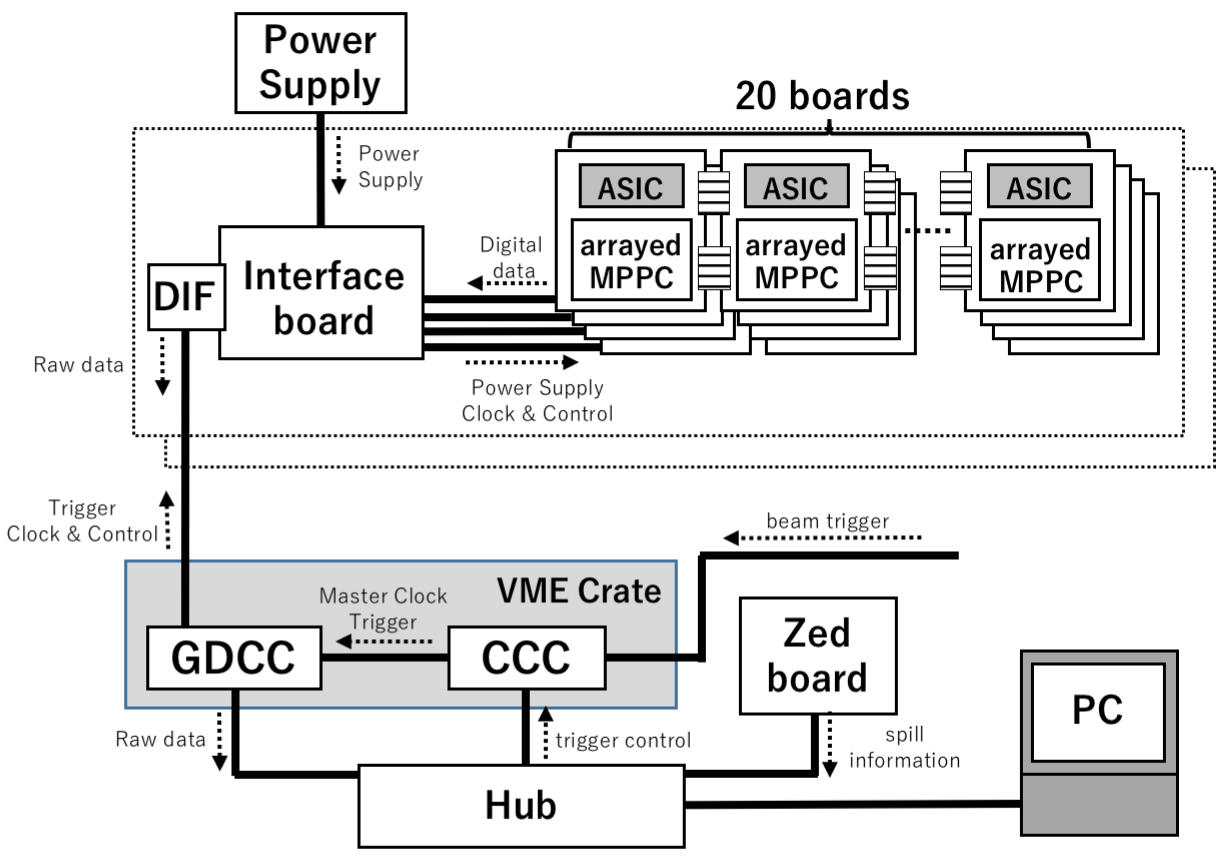
\includegraphics[width=0.7\linewidth]{DAQ-schematics}
  \caption{The schematics of the WAGASCI DAQ system. The very same schematics
    can be referred to the SideMRD where instead of 20 boards there are only 3
    and instead of arrayed MPPCs there are Single MPPCs
    adapters}\label{DAQ-schematics}
\end{figure}

\subsection{References}
The documentation about the WAGASCI electronics is relatively vast but randomly
dispersed through the net. Here I am providing a compilation of all the
available literature that I could find.

\begin{itemize}
\item Master Theses about the WAGASCI electronics and DAQ system: Chikuma
  Naruhiro~\cite{Chikuma:2016}, Tamura Riku~\cite{Tamura:2018}.
\item Articles about the WAGASCI electronics (but not directly referring to the
  WAGASCI experiment):~\cite{Gastaldi:2014vaa,Gastaldi:2014oid,GDCC:2012}.
\item General articles about pre-amplifiers and amplifiers used for Physics
  measurements~\cite{Hamamatsu:2001,Bertuccio:1996,Lioliou:2015,Ortec} and
  everything about signal processing that you can find in the Knoll
  book~\cite{Knoll:2010radiation}. This should be enough to get you started. Of
  course there is much more online about Physical applications of pre-amplifier
  and amplifiers.  
\item Articles and slide shows about the SPIROC
  characterization~\cite{Callier:2008,Callier:2009,Fabbri:2009,%
    Callier:2013,Callier:2015}.
\item SPIROC manuals and
  pin-out~\cite{SPIROC2Dpinlist,SPIROC2Ddatasheet,SPIROC:OMEGA}.
\end{itemize}

\section{SPIROC2D}
The SPIROC2D chip can be considered as the heart of the WAGASCI DAQ system. It
is directly connected to the MPPCs and plays the role of pre-amplifier,
amplifier and digitalization of the raw signal. It is contained in an ASIC
called \hyperref[sec:ASU]{ASU} (Section~\ref{sec:ASU}). In
Figure~\ref{DAQ-schematics} it is indicated with the general term ASIC.

SPIROC is a dedicated very front-end chip developed originally for an ILC
prototype hadronic Calorimeter with SiPM readout (CALICE experiment). It has
been realized in 0.35$\mu$m SiGe technology. It has been developed to match the
requirements of large dynamic range, low noise, low consumption, high precision
and large number of readout channels needed. The SPIROC version used for the
WAGASCI DAQ is SPIROC2D.

The SPIROC ASIC that reads 36 SiPMs is an evolution of the FLC\_SiPM used in the
CALICE experiment prototype. The first SPIROC prototype has been produced in
June 2007 and packaged in a CQFP240 package. A second version, SPIROC2, was
realized in June 2008 to accommodate a thinner TQFP208 package and fix a bug in
the ADC.

SPIROC is an \textbf{auto-triggered} (it is possible to set a threshold value
below which no data is acquired), \textbf{bi-gain} (there are two pre-amplifiers
one with low gain for bigger signals and another with higher gain for smaller
signals), \textbf{36-channel} ASIC which allows to measure on each channel the
charge from one photoelectron to 2000 and the time with a 100ps accurate TDC (be
warned that accuracy and precision are two distinct concepts).\@ An analog
memory array (Switched Capacitor Array) with a depth of 16 for each is used to
store the time information and the charge measurement. Refer to Wikipedia for
more info about the SCA (this should be more than enough if you are an
experimental physicist like me).

A 12-bit Wilkinson ADC has been embedded to digitize the analog memory contents
(time and charge on 2 gains). The data are then stored in a 4 kilobytes RAM.\@ A
very complex digital part has been integrated to manage all theses features and
to transfer the data to the DAQ.\@

A small list of the most basic SPIROC properties:
\begin{itemize}
\item ASIC name: SPIROC (Silicon PM Integrated Read-Out Chip)
\item Current available version: 2A,2B,2C,2D,2E
\item Number of channel: 36
\item Polarity of input signal: positive
\item Detector read out: SIPM, MPPC, compliant with PM, MA-PM
\item Max input signal: 2000 photoelectrons at minimum gain
\end{itemize}

\subsection{Short description}
Please read this section only after having read at least some of the references
above otherwise it probably won't make much sense.

Each channel of SPIROC2 is made of:
\begin{itemize}
\item An 8-bit input DAC with a very low power of 1$\mu$W/channel as it is not
  power pulsed. The DAC also has the particularity of being powered with 5V
  whereas the rest of the chip is powered with 3.5V. Think of this DAQ as a way
  to fine tune the High Voltage supplied to the MPPCs in a range from -4V to
  +4V. TO-CHECK the range. This tuning directly reflects on the gain of that
  particular channel. It is possible to control this value by tweaking the TO-DO
\item A high gain and a low gain pre-amp in parallel on each input allow
  handling the large dynamic range. A gain adjustment over 6 bits common for the
  64 channels has been integrated in SPIROC2. TO-CHECK it is not clear!
\item The charge is measured on both gains by a ``slow'' shaper (an amplifier
  with pulse duration of 50–150ns) followed by an analogue memory (SCA) with a
  depth of 16 capacitors.
\item The auto-trigger is taken on the high gain path with a high-gain fast
  shaper followed by a low offset discriminator. In other words the input signal
  is first processed by the high-gain pre-amp and then compared with a given
  threshold (that can be adjusted). If the signal is ``over'' the threshold the
  acquisition is triggered, otherwise the signal is ignored. By low offset I
  mean that (due to a hardware error) the threshold is not set on the main part
  of the pulse but on the lower part of the pulse as one can see in
  figure~\ref{threshold-bug}. This erroneous behavior has been fixed in the
  SPIROC2E version but it has been shown that it doesn't affect the measure so
  much as to require a replacement of all the chips.
  \begin{figure}[ht]
    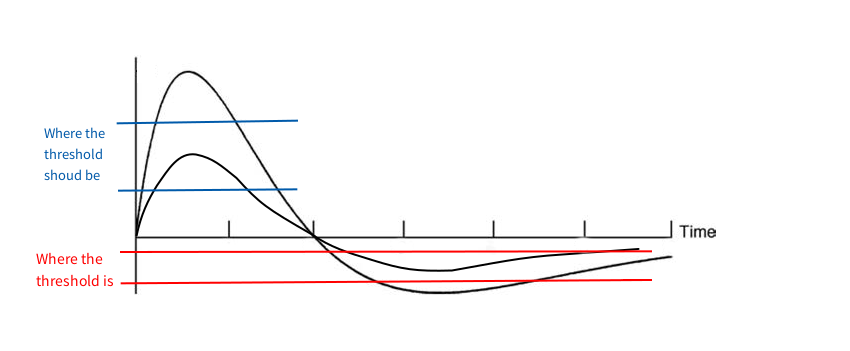
\includegraphics[width=\linewidth]{threshold-bug.png}
    \caption{The threshold should be applied on the upper part of the signal and
      not on the lower. This figure shows two signals over the respective
      thresholds. The blue lines show where the threshold should be: in this
      case only signal ABOVE the threshold value trigger acquisition. The red
      lines show where the threshold actually is: in this case only signals
      BELOW the threshold value trigger acquisition.}\label{threshold-bug}
  \end{figure}
  The discriminator output is used to generate the hold-and-track on the 36
  channels. The threshold is common to the 36 channels, given by a 10 bit DAC
  with a subsequent 4 bit fine tuning per channel.
\item The discriminator output is also used to store the value of a 300ns ramp
  in a dedicated analogue memory to provide time information with an accuracy of
  100 ps.
\item A 12 bit Wilkinson ADC is used to digitize the data at the end of the
  acquisition period.
\end{itemize}
The digital part is complex as it must handle the SCA write and read pointers,
the ADC conversion, the data storage in a RAM and the readout process.

The chip has been extensively tested by many groups. The first series of tests
has been mostly devoted to characterizing the analog performance, which meets
the design specifications.

\subsection{ASU}\label{sec:ASU}
\begin{figure}[ht]
  \centering 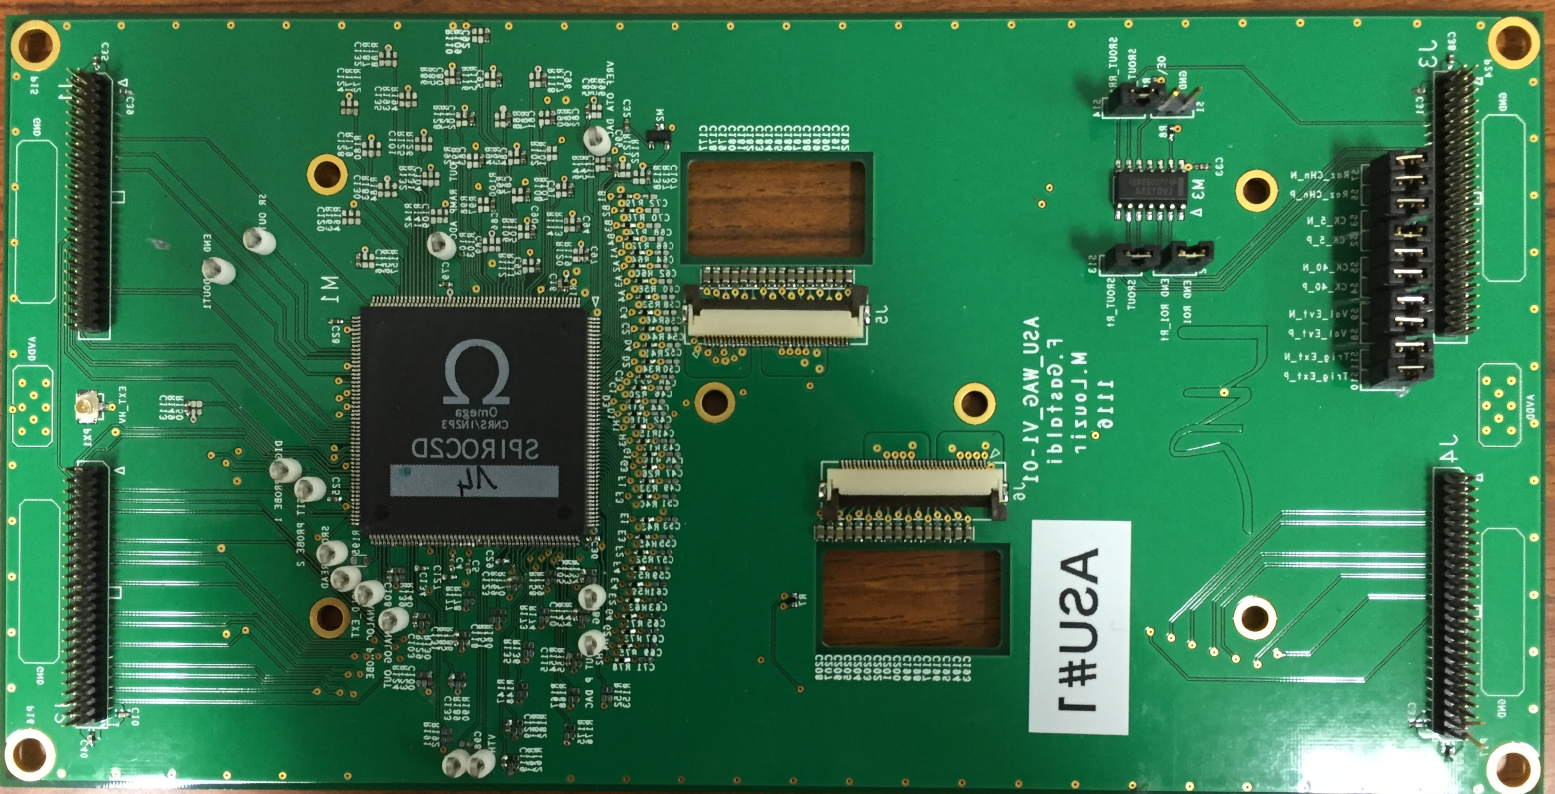
\includegraphics[width=0.8\linewidth, frame]{ASU}
  \caption{Active Sensor Unit (ASU) board}
\end{figure}
Active Sensor Unit (ASU) board is the name of the PCB board containing the
SPIROC2D chip. It is basically an adapter to connect the SPIROC chip to the
MPPCs and to the rest of the DAQ system. The ASUs can be daisy-chained together
until a maximum of 40 units (4 rows of 5 ASUs) for every DIF, as can be seen in
Figure~\ref{daisy-chain}.
\begin{figure}[ht]
  \centering 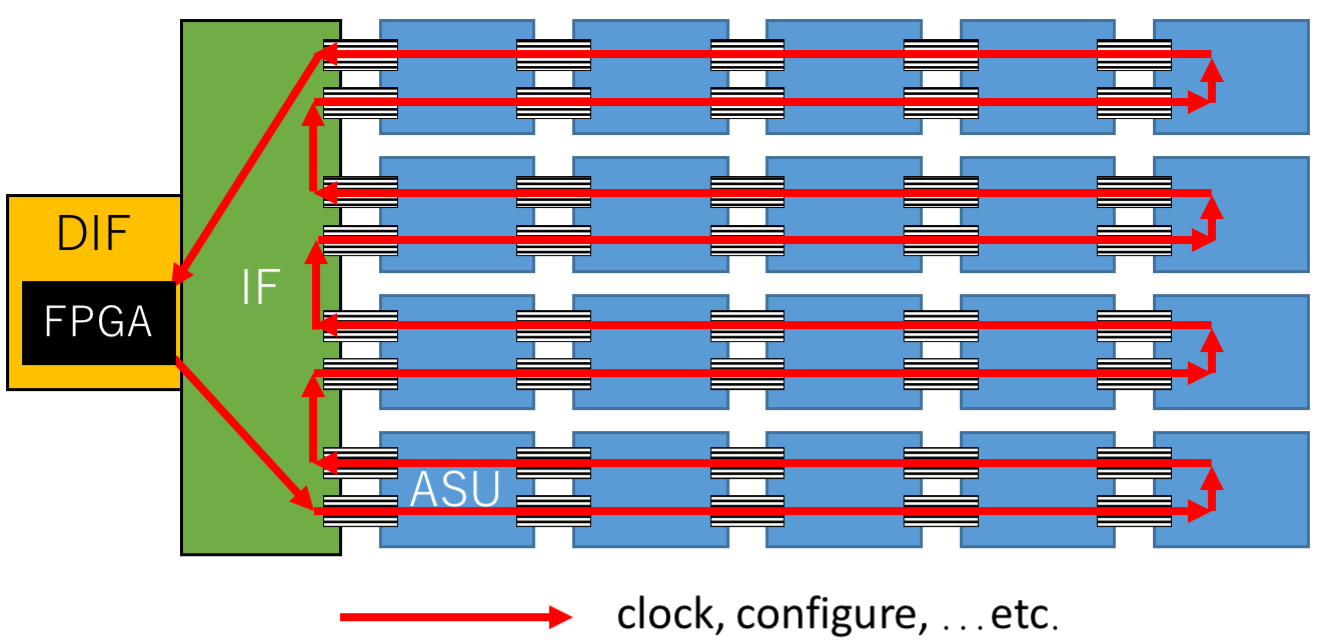
\includegraphics[width=0.7\linewidth]{daisy-chain}
  \caption{Schematic of ASU daisy chain}\label{daisy-chain}
\end{figure}
The jumpers of the last ASU of every row must be set as shown in
Figures~\ref{fig:ASU-with-jumpers},~\ref{fig:ASU-without-jumpers}
and~\ref{ASU-daisy-chain} to reflect the signal back to the interface.
\begin{figure}[ht]
  \centering
  \begin{minipage}{0.5\linewidth}
    \centering 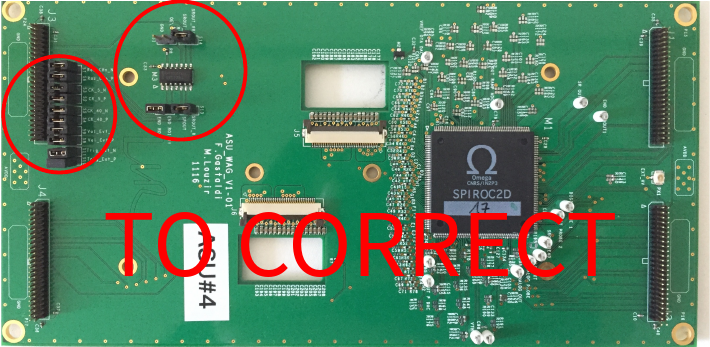
\includegraphics[width=0.98\linewidth,frame]{ASU-with-jumpers}
    \caption{ASU with jumpers}\label{fig:ASU-with-jumpers}
  \end{minipage}%
  \begin{minipage}{0.5\linewidth}
    \centering 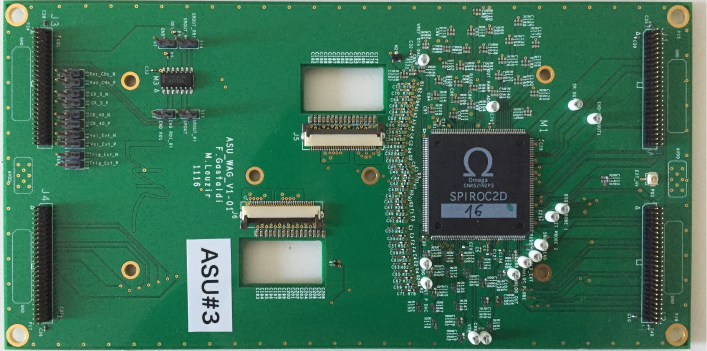
\includegraphics[width=0.98\linewidth,frame]{ASU-without-jumpers}
    \caption{ASU without jumpers}\label{fig:ASU-without-jumpers}
  \end{minipage}
\end{figure}
\begin{figure}[ht]
  \centering 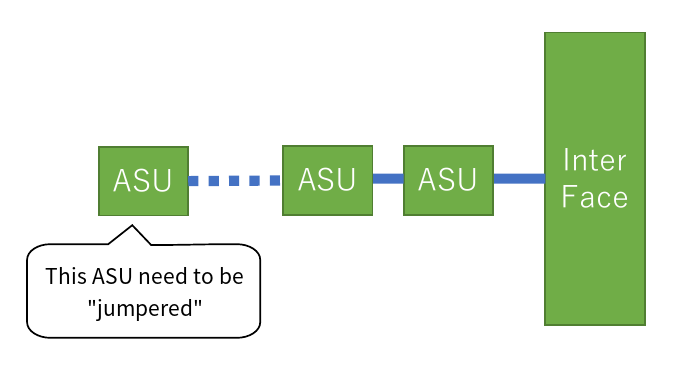
\includegraphics[width=0.5\linewidth, frame]{ASU-daisy-chain}
  \caption{How to daisy chain and jumper the last ASU of the row.}%
  \label{ASU-daisy-chain}
\end{figure}

Moreover, pay attention when you connect the ASUs to the interface because it is
not as straightforward as it seems. As can be seen in
Figure~\ref{fig:ASU-Interface1}, it can happen that the cables cross. Notice
also that the bump in the cable have to correspond to the silkscreen prints on
the circuit. Anyway, you can refer to table~\ref{tab:ASU-IF} for the ASU-IF
connections.
\begin{table}[H]
  \centering \bgroup
  \def\arraystretch{1.5}% 1 is the default, change whatever you need
  \begin{tabular}{|c|c|c|c|c|}
    \hline
    & \textbf{ASU 1} & \textbf{ASU 2} & \textbf{ASU 3} & \textbf{ASU 4} \\
    \hline
    \textbf{ASU connector} & J1 J2 & J1 J2 & J1 J2 & J1 J2  \\
    \hline
    \textbf{IF connector} & J2 J5 & ? & ? & ?  \\ % chktex-file 26
    \hline
  \end{tabular}
  \egroup
  \caption{ASU - Interface connections}\label{tab:ASU-IF}
\end{table}
\begin{figure}[ht]
  \centering
  \begin{minipage}{0.4\linewidth}
    \centering 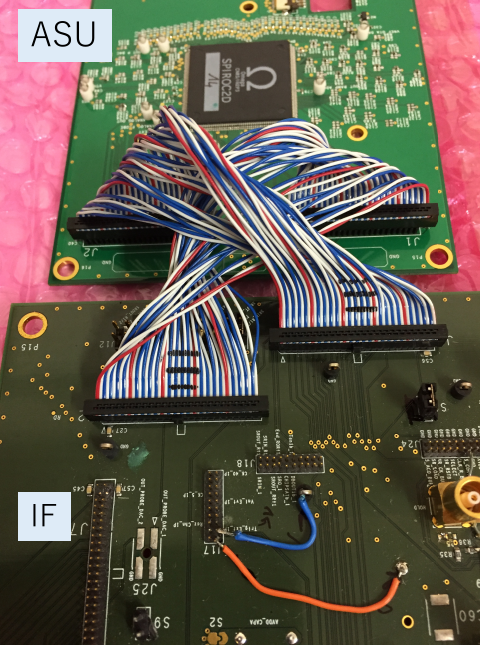
\includegraphics[width=0.9\linewidth,frame]{ASU-Interface1}
    \caption{Pictures the flat cables that connect an ASU to its
      Interface}\label{fig:ASU-Interface1}
  \end{minipage}%
  \begin{minipage}{0.5\linewidth}
    \centering \includegraphics[width=0.9\linewidth,frame]{ASU-Interface2}
    \caption{Close view of the connectors}\label{fig:ASU-Interface2}
  \end{minipage}
\end{figure}


\section{Interface}
\begin{figure}[H]
  \centering 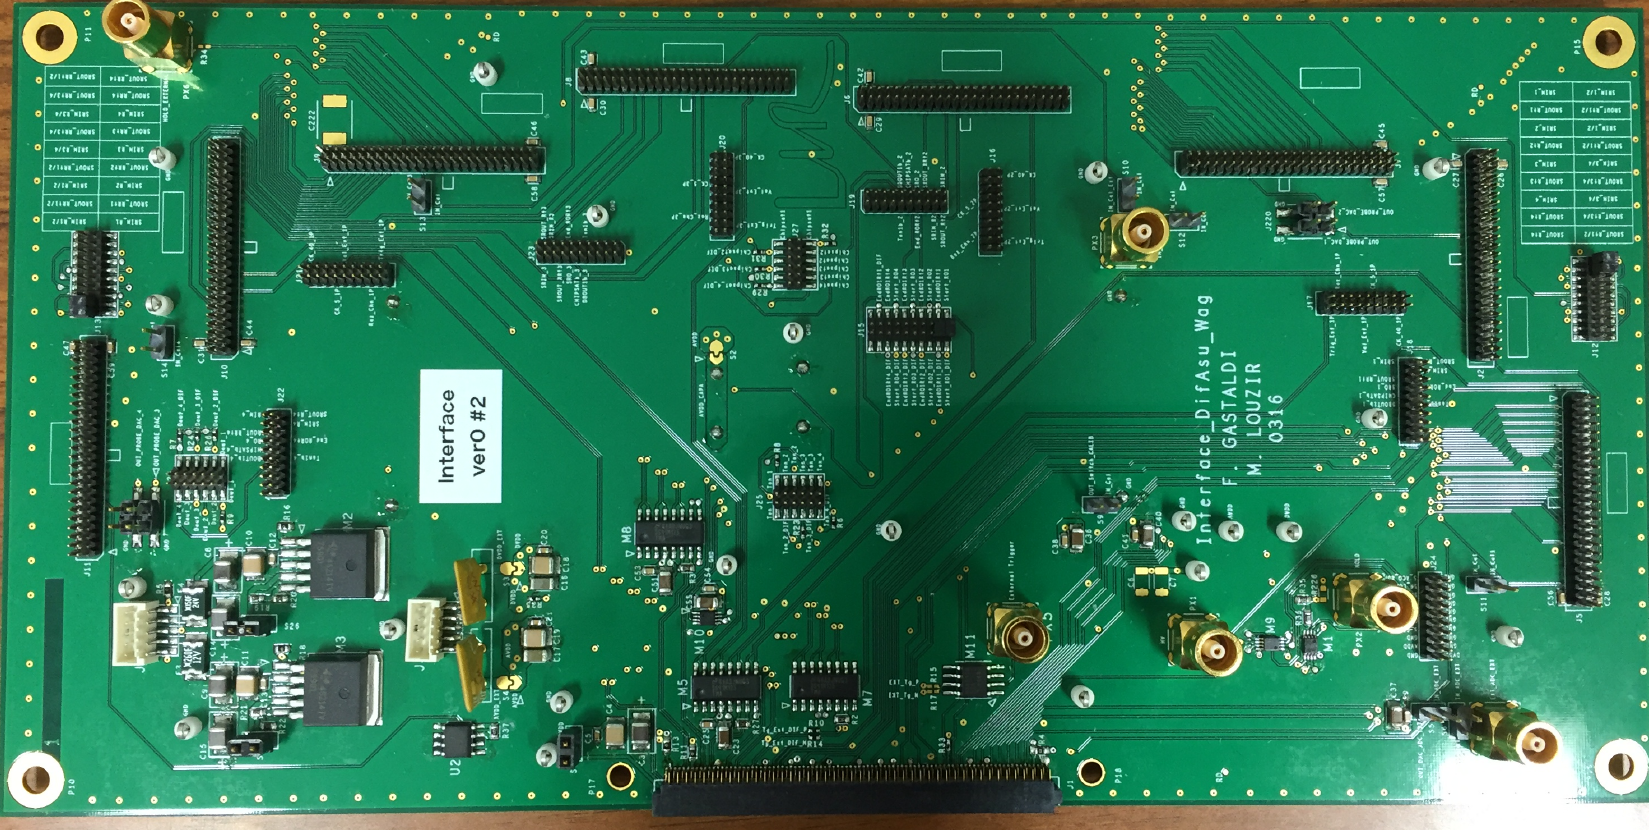
\includegraphics[width=0.8\linewidth, frame]{Interface}
  \caption{Interface (before buffer addition)}\label{fig:Interface}
\end{figure}
This board has no important function by itself. It is just a sort of adapter to
connect all the ASUs to the DIF, to route the High Voltage to the MPPCs (through
the SPIROC2C chip) and to route the Low Voltage to the SPIROC2D chip itself and
to the DIF. Despite being the most trivial board of the system it is the
component that gave more problems in the past.

The connectors are quite fragile and I counted at least 5 boards broken when
disconnecting some cables (including one by myself). In particular take extra
care when connecting-disconnecting the DIF and the Low Voltage.

The High voltage must be connected to the only LEMO 00 female connector that can
be seen on the right of the DIF in Figure~\ref{fixed-interface}. Where to
connect the Low Voltage cable is shown in Figure~\ref{low-vol-pin-out} and in
Section~\ref{sec:how-make-low-voltage-cable}.

The Interface shown if Figure~\ref{fig:Interface} is just a prototype (before
the patch described in Section~\ref{sec:how-patch-interface} is applied). The
actual Interface board may look different.

\subsection{How to patch the interface}\label{sec:how-patch-interface}
As can be read in Tamura Riku's thesis (after correcting some typos):

\textit{[\dots] in order to check the correct operation of the full setup, the
  daisy chain configuration is firstly tested. The test is done by increasing
  the number of daisy-chained ASU boards one by one. Up to about 10 boards, the
  daisy chain is correctly configured but at around 10 boards the configuration
  starts to fail. After several tests with different configurations, it appeared
  that this is due to the attenuation and reflection of the bunch crossing clock
  (BCID) when it travels through the chain: the signals, including the bunch
  crossing clock, are serially transported through the daisy chain so the length
  that they need to travel depends on the number of connected ASU boards. The
  total capacitance of the daisy chain depends on the number of connected ASU
  boards, too. This creates a mismatch of impedance between the endpoints and
  some DAQ signals are badly affected. In practice most of the DAQ signals are
  not so affected but it seems that the bunch crossing clock is strongly
  affected. The whole DAQ acquisition phase is synchronized to the bunch
  crossing clock so this is a very critical issue.}

\textit{Fortunately, this problem can be fixed by ``patching'' the bunch
  crossing clock line. To prevent the attenuation of bunch crossing clock and
  match the impedance a 4ch buffer,
  CDCLVC1104\cite{Texas-Instruments:CDCLVC11xx}, is applied to the bunch
  crossing clock line as shown in Figure TO-DO. This buffer is a highly
  performing and fast responding one. The delay it adds to the BCID is of
  0.8-2ns, which is less than 1\% of the period of bunch crossing clock, so the
  effect on the timing measurement due to the BCID is negligible. This patch is
  tested to work fine and the daisy chain is configured correctly even with the
  full setup (20 ASUs). [\dots]}

Long story short, we have to patch every interface with that chip if we want to
daisy-chain more than 10 ASUs. Just to be on the safe side, all the interface
boards, even if connected to less than 10 ASUs, were fixed with the following
procedure.

Here I will show how to concretely fix the interface. I came to know about this
procedure by reading two pdf files that were sent to YNU from I don't know
where. I must admit that until now they hold the record for being the most
unintelligible piece of paper that I have ever read. No matter how much I
strove, I think that I could never write in such a cumbersome manner even if I
want to. Anyway \dots
\begin{enumerate}
\item First solder the CDCLVC1104 chip on the base and glue it on the board (any
  empty space on the interface is good) as shown in Figure~\ref{buffer}. You can
  use a different support (the white piece of plastic) and base (the small PCB
  with 10 holes on each side) if you want.
  \begin{figure}[H]
    \centering 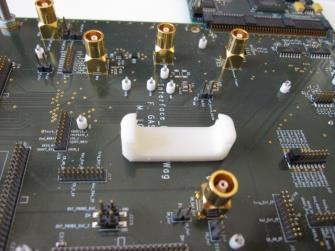
\includegraphics[frame,width=.3\textwidth]{support}\hfill
    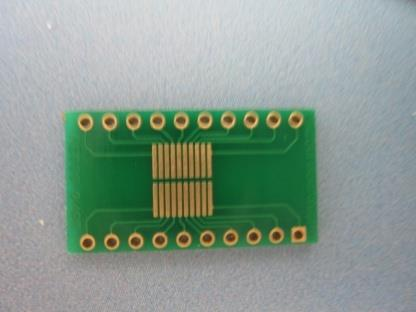
\includegraphics[frame,width=.3\textwidth]{base}\hfill
    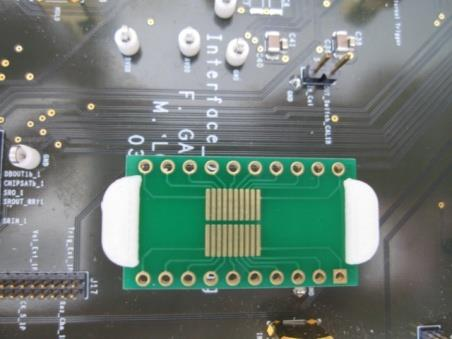
\includegraphics[frame,width=.3\textwidth]{base-glued}
    \caption{PCB Base (in the middle) glued to the interface board using a
      plastic support (on the left). The buffer chip must be soldered on that
      base (not shown in the pictures, yet). You can solder the buffer chip in
      any position on the base as long as it is soldered
      properly.}\label{buffer}
  \end{figure}
\item Then take a 50 pins flat cable (that you are then going to connect to the
  J2 connector). Cut in the middle the wires number 13, 49 and 50 (SR\_CK\_BUF,
  TRIG\_EXT\_N and TRIG\_EXT\_P respectively). Refer to Figure~\ref{J2} for the
  flat cable pin-out. Strip the ``ASU end'' of these wires. By ASU end I mean
  the end that is not to be connected to the interface but to the ASU. If needed
  do the same for the other flat cables coming out the connectors J6, J8 and
  J10.
  \begin{figure}[H]
    \centering 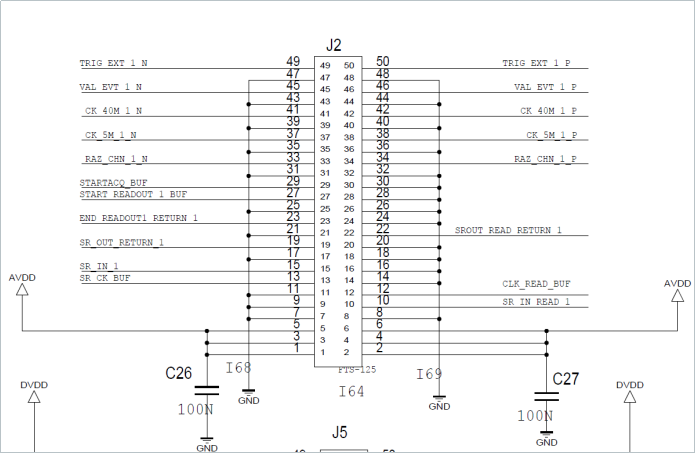
\includegraphics[frame,width=0.7\linewidth]{J2}
    \caption{J2 connector pin-out}\label{J2}
  \end{figure}
\item Desolder the M9 chip
  \begin{figure}[H]
    \centering 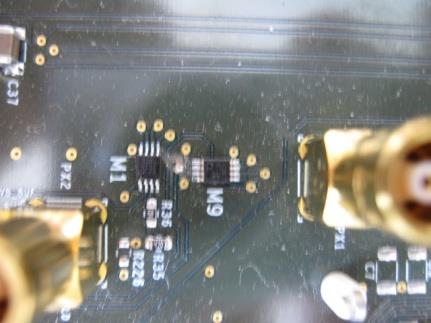
\includegraphics[frame,width=0.5\linewidth]{desolder}
    \caption{CDCLVC1104 chip pin-out}\label{desolder}
  \end{figure}
\item Referring to Figures~\ref{interface-connections}
  and~\ref{buffer-blueprint}, connect with some wires the pins in this way:
  \begin{table}[H]
    \centering \bgroup
    \def\arraystretch{1.5}% 1 is the default, change whatever you need
    \begin{tabular}{|c|c|c|}
      \hline
      \textbf{color} & \textbf{CDCLVC1104 pin} & \textbf{Interface pin} \\
      \hline
      brown & 1 CLKIN & SR\_clk \\
      \hline
      red & 6 VDD & (refer to picture) \\
      \hline
      black & 4 ground & Interface ground \\
      \hline
    \end{tabular}
    \egroup
    \caption{Fast command packet format}
  \end{table}
  \begin{figure}[H]
    \centering 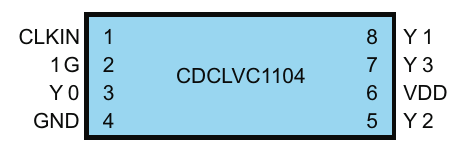
\includegraphics[width=0.7\linewidth]{buffer-blueprint}
    \caption{CDCLVC1104 chip pin-out}\label{buffer-blueprint}
  \end{figure}
  \begin{figure}[H]
    \centering
    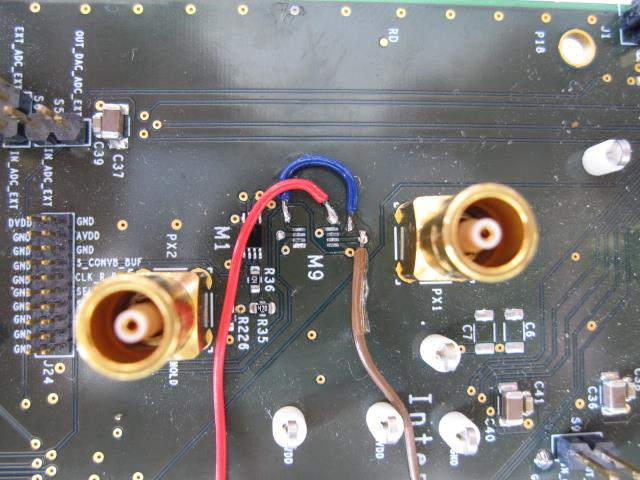
\includegraphics[frame,width=.3\textwidth]{interface-pinout1}\hfill
    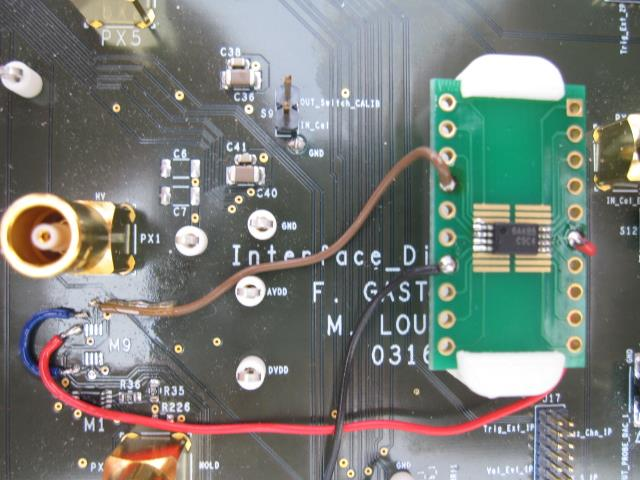
\includegraphics[frame,width=.3\textwidth]{interface-pinout2}\hfill
    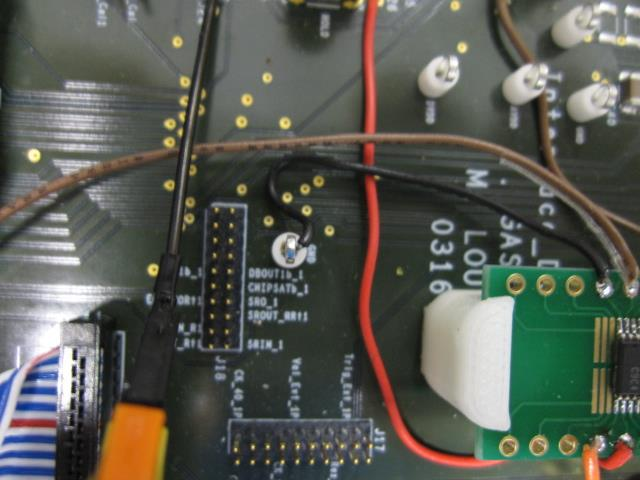
\includegraphics[frame,width=.3\textwidth]{ground}
    \caption{Interface connections}\label{interface-connections}
  \end{figure}
  I am sorry but in the document that I was given there is no schematics
  regarding the holes around the M9 chip, so we had to solder referring only to
  the attached pictures.
\item (Optional but recommended) Solder a capacitor of 100nf to decouple power
  and ground between the pins 6 VDD and 4 GRD of the buffer. It is not shown in
  the pictures.
\item Now connect the interface holes around the M9 chip as shown in
  Figures~\ref{interface-connections} (blue cable). In the document I was given
  those are called pin number 1 and 7. Anyway, as I said, without the schematics
  those numbers are meaningless. Sometimes I wonder if Physicists are really so
  smart as they think to be.
\item Pins 3,5,7,8 of the buffer chip represent the output of the
  buffer. Connect each pin to the wire number 13 of the flat cables coming off
  J2, J6, J8 and J10. The order is not relevant. Of course, in the case of the
  SideMRD, only one connection is needed (for example J2). Refer to
  Figure~\ref{connection_flat_cable} for a visual explanation.
  \begin{figure}[H]
    \centering 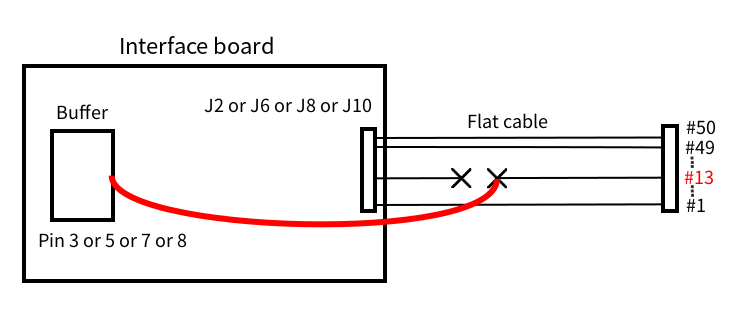
\includegraphics[width=0.6\linewidth]{connection_flat_cable}
    \caption{How to connect the \#13 wire to the buffer.}%
    \label{connection_flat_cable}
  \end{figure}
\item Connect wire number 50 of the flat cable (it is white in our case) to any
  ground pin on the interface board. You have to connect the ``ASU end'' of the
  wire to ground in a similar way as shown in Figure~\ref{connection_flat_cable}
  for the case of cable 13.
\item Connect wire number 49 of the flat cable (it is blue in our case) to the
  DVD pin on the interface board. The DVD pin is located near the M9 chip that
  you just desoldered. You have to connect the ``ASU end'' of the wire to the
  DVD pin in a similar way as shown in Figure~\ref{connection_flat_cable} for
  the case of cable 13.
\item The final result should look more or less like
  Figure~\ref{fixed-interface}.
  \begin{figure}[ht]
    \centering \includegraphics[frame,width=0.9\linewidth]{fixed-interface}
    \caption{Final result. Notice that the ground wire coming from wire 50 of
      the flat cable is ambiguously red and not black as it should be. The green
      wire is coming off from wire number 49 and is connected to the DVD pin on
      the Interface. In total there are three yellow output wires coming off the
      buffer chip but only one is actually used.}\label{fixed-interface}
  \end{figure}
\end{enumerate}

\subsection{How to make a Low Voltage cable}\label{sec:how-make-low-voltage-cable}
For bench-testing purposes you may need to make your own Low Voltage cable to
power the Interface and all the other boards connected to it.

The Low Voltage cable must be connected to the interface using a 5 pins
connector to a vertical wire-to-board socket that looks like this:
\begin{figure}[H]
  \centering
  \begin{minipage}{0.15\linewidth}
    \centering 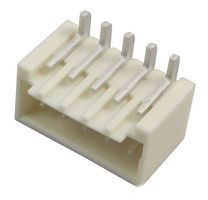
\includegraphics[width=\linewidth,frame]{low-vol-socket1}
  \end{minipage}%
  \begin{minipage}{0.6\linewidth}
    \centering 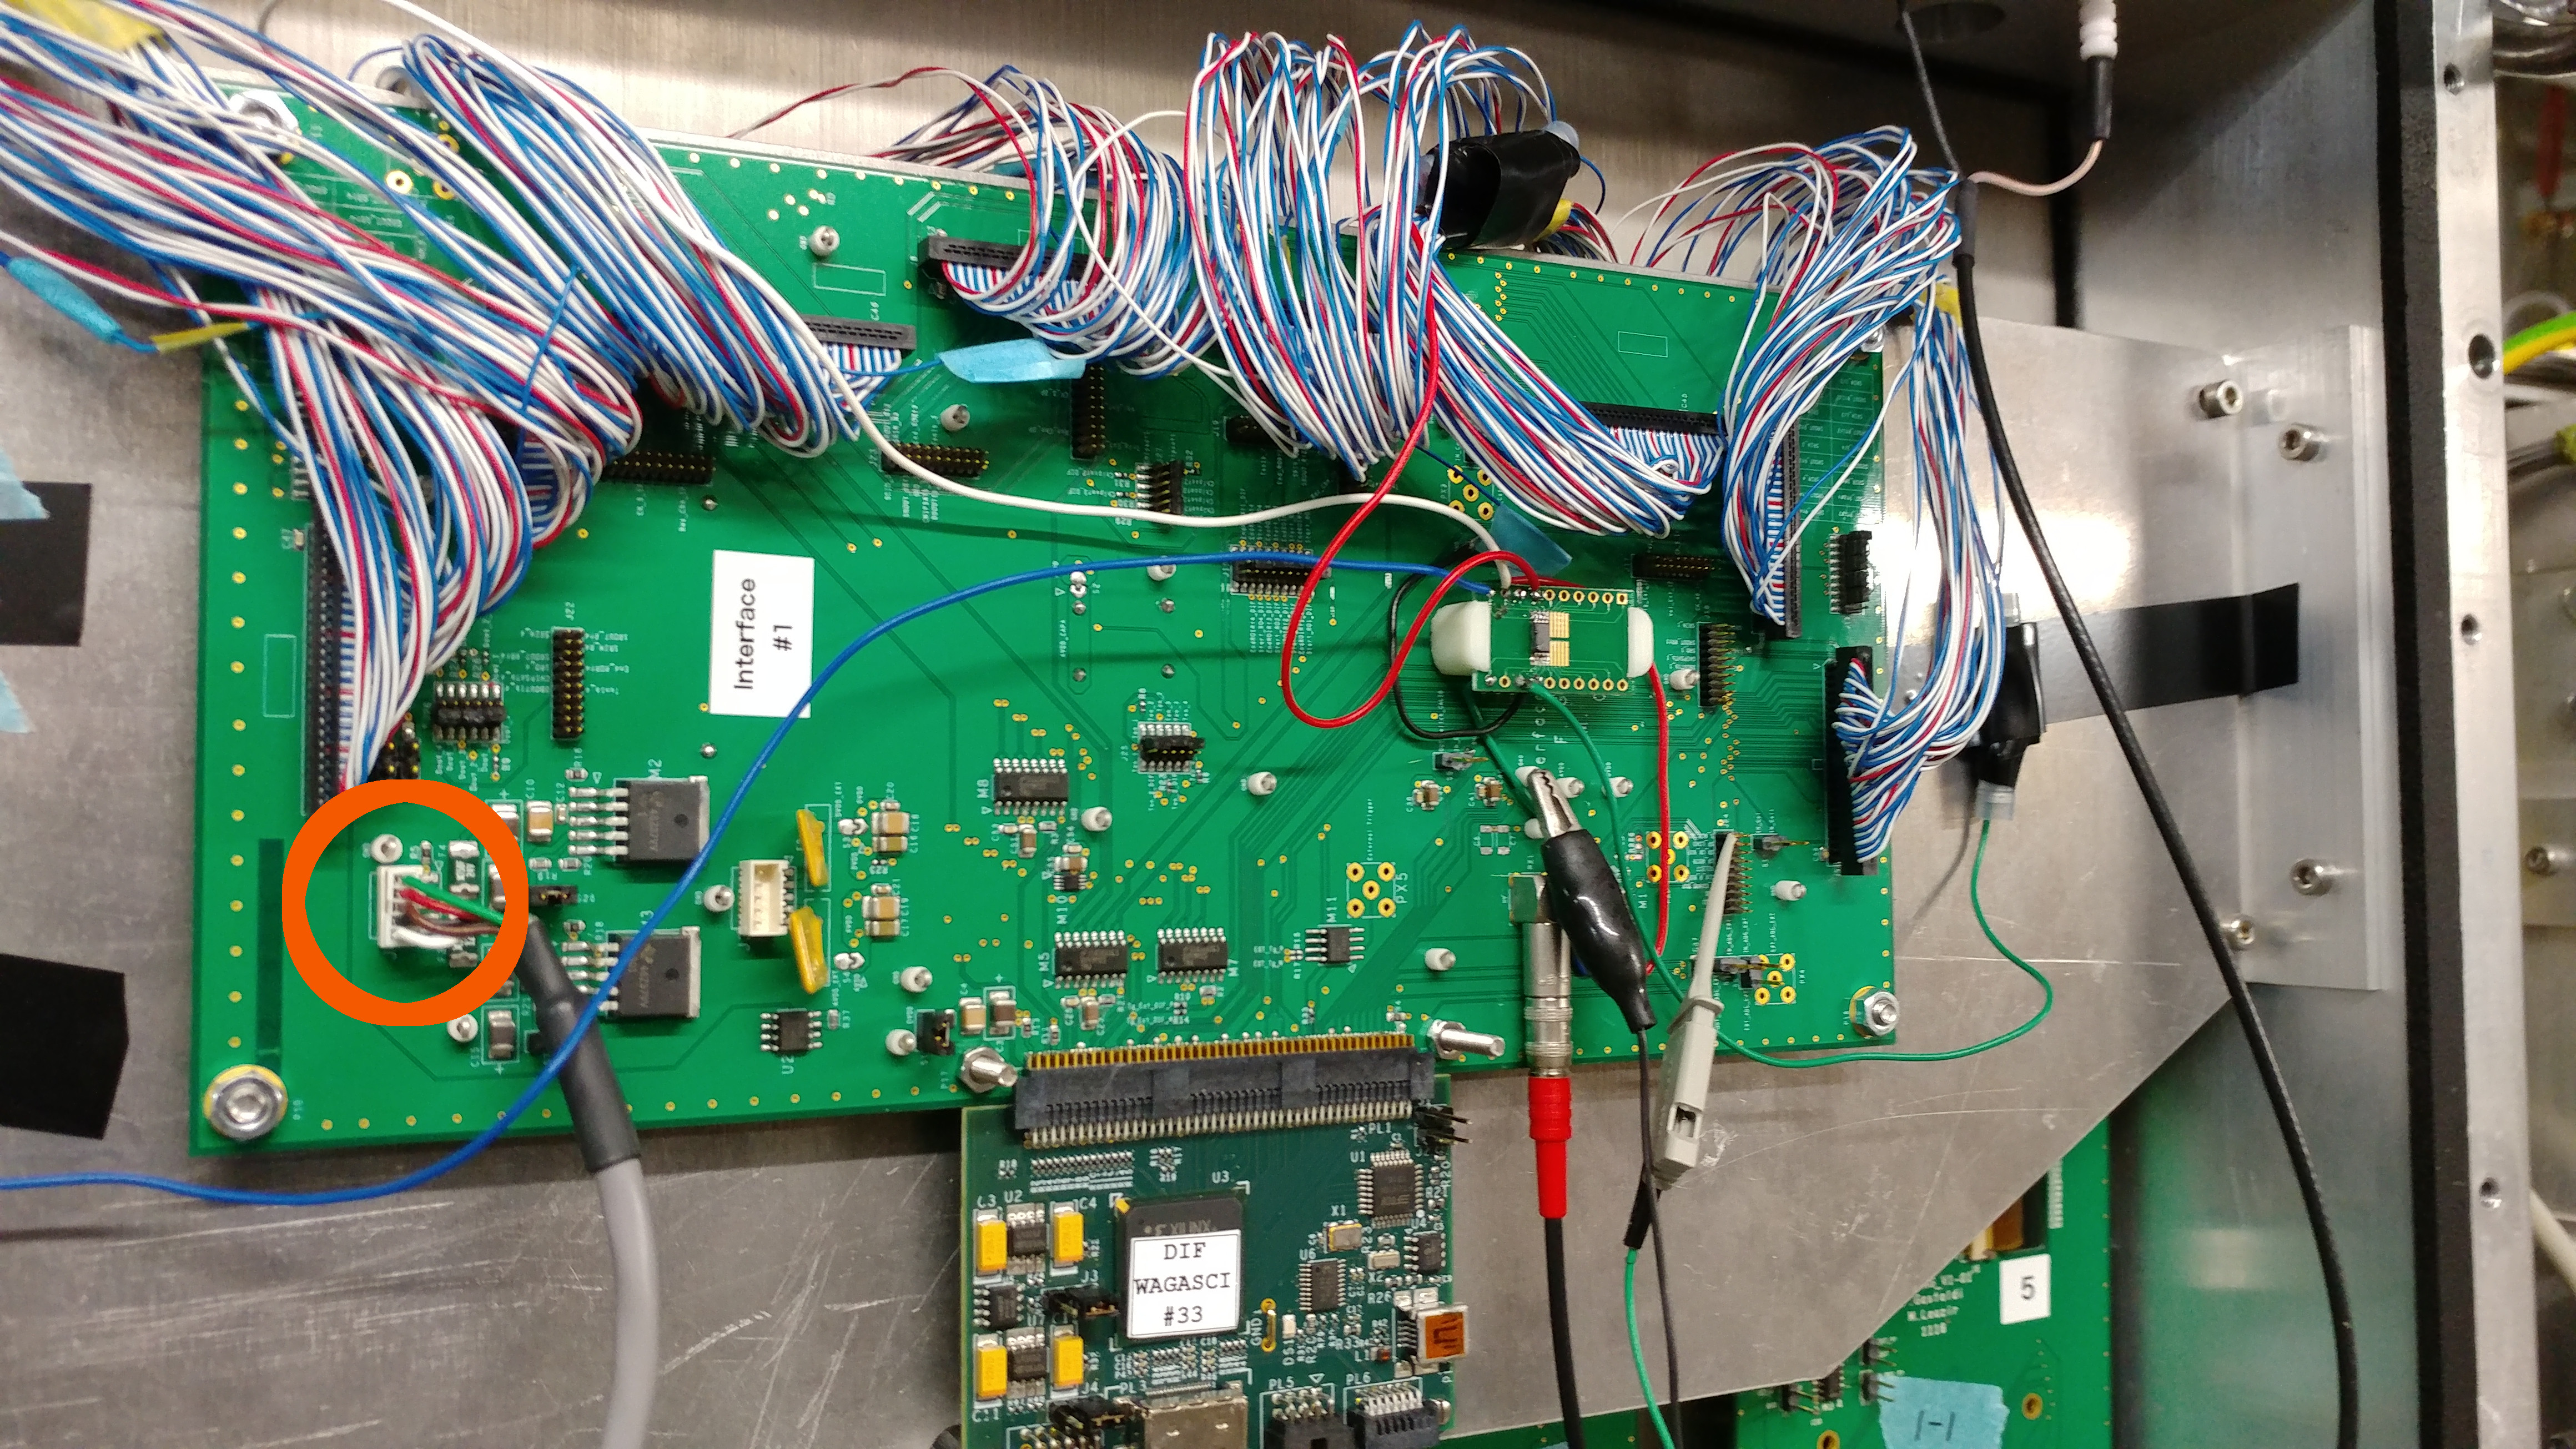
\includegraphics[width=0.9\linewidth,frame]{low-vol-socket2}
  \end{minipage}
  \caption{Vertical wire-to-board 5-pins socket on the Interface board for the
    Low Voltage connection}\label{low-vol-socket}
\end{figure}
To make the cable just buy a male connector (TO-DO insert link) and connect the
pins following the pin-out of Figure~\ref{low-vol-pin-out}.
\begin{figure}[H]
  \centering 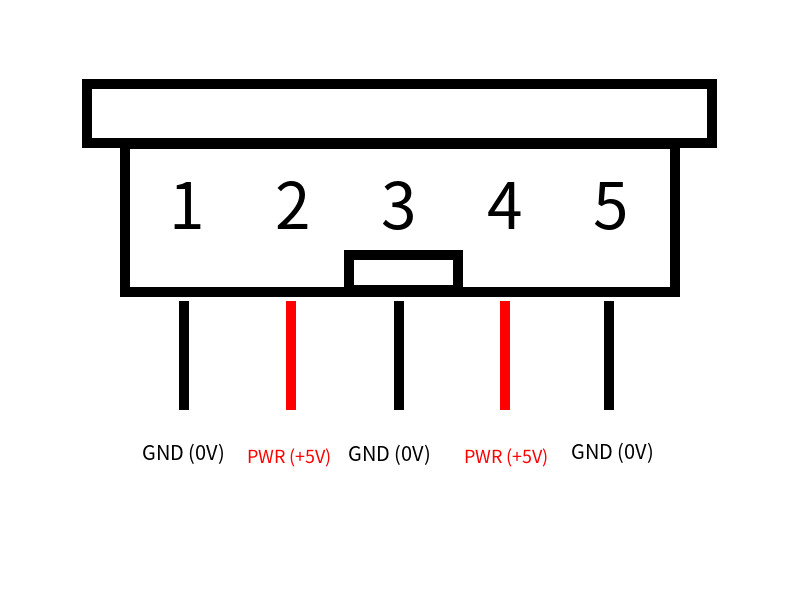
\includegraphics[width=0.5\linewidth]{low-vol-pin-out}
  \caption{Vertical wire-to-board 5-pins socket on the Interface board for the
    Low Voltage connection}\label{low-vol-pin-out}
\end{figure}
The ground wires can be grouped together in a single wire. The 5V wires can be
grouped together in a single wire, too. The resulting 2 wires end of the cable
can be terminated as you like and then connected to a 5V power supply. The power
supply should be able to generate at least TO-DO Amperes of current.

\section{DIF}
I have not much to say about the Detector InterFace (DIF) board. It converts the
signal from the ASUs into HDMI and sends it to the GDCC. It also controls the
synchronization and reset of the slow clock (BCID). Until present there were
many issues related to the slow-clock reset and synchronization, all of which
have been luckily solved by a DIF firmware upgrade. To know more about the DIF
please contact Matsushita Kouhei (Tokyo University): he was the one that tested
the new firmware. To flash the updated firmware refer to Section TO-DO

Remember to note down the port number (Figure~\ref{fig:GDCC-front-view}) on the
GDCC side that you connect each DIF to, because you will have to insert that
number in the configuration file TO-DO.
\begin{figure}[H]
  \centering
  \begin{minipage}{0.2\linewidth}
    \centering 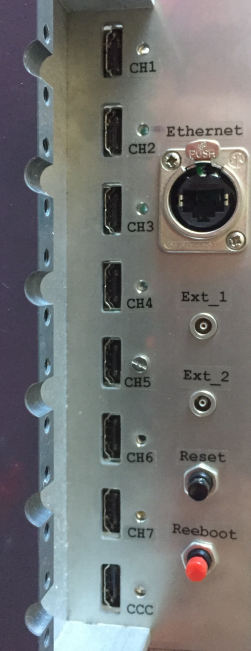
\includegraphics[width=0.9\linewidth, frame]{GDCC-front-view}
    \caption{GDCC front view}\label{fig:GDCC-front-view}
  \end{minipage}%
  \begin{minipage}{0.7\linewidth}
    \centering 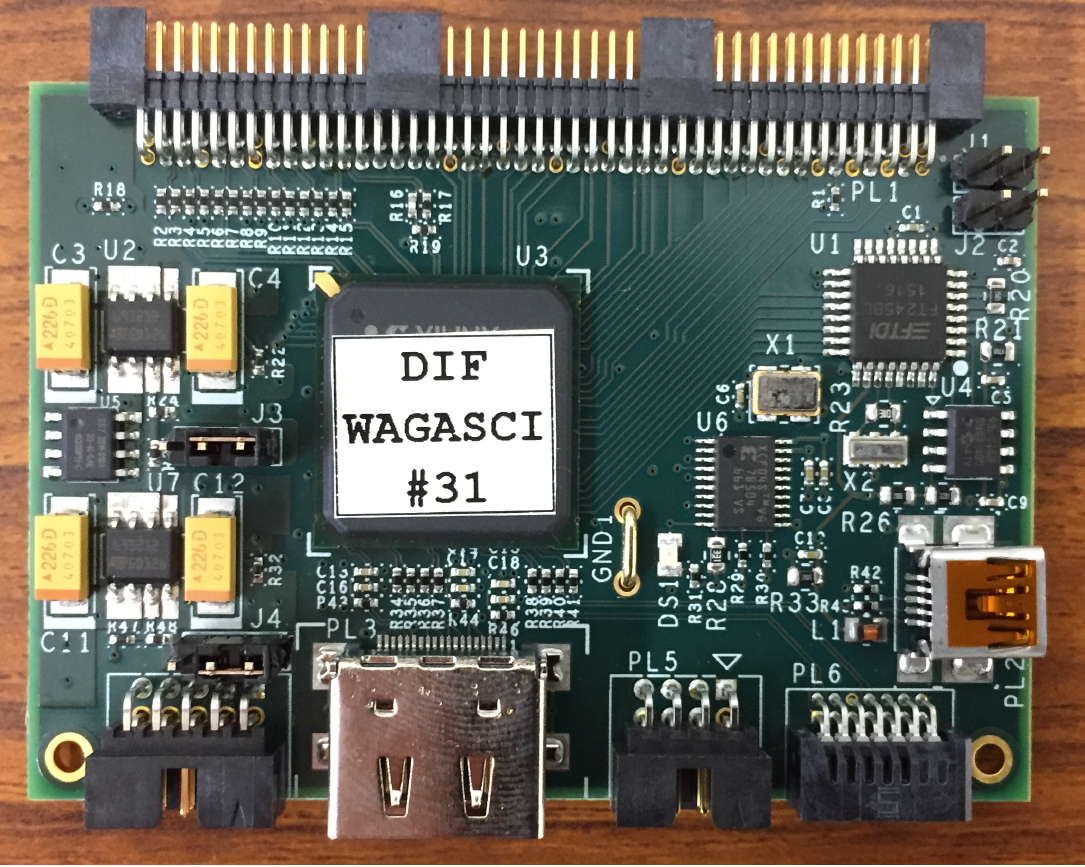
\includegraphics[width=0.9\linewidth, frame]{DIF}
    \caption{Detector InterFace (DIF)}
  \end{minipage}
\end{figure}

\subsection{DIF Firmware upgrade}

TO-DO

\section{GDCC}
\begin{figure}[ht]
  \centering 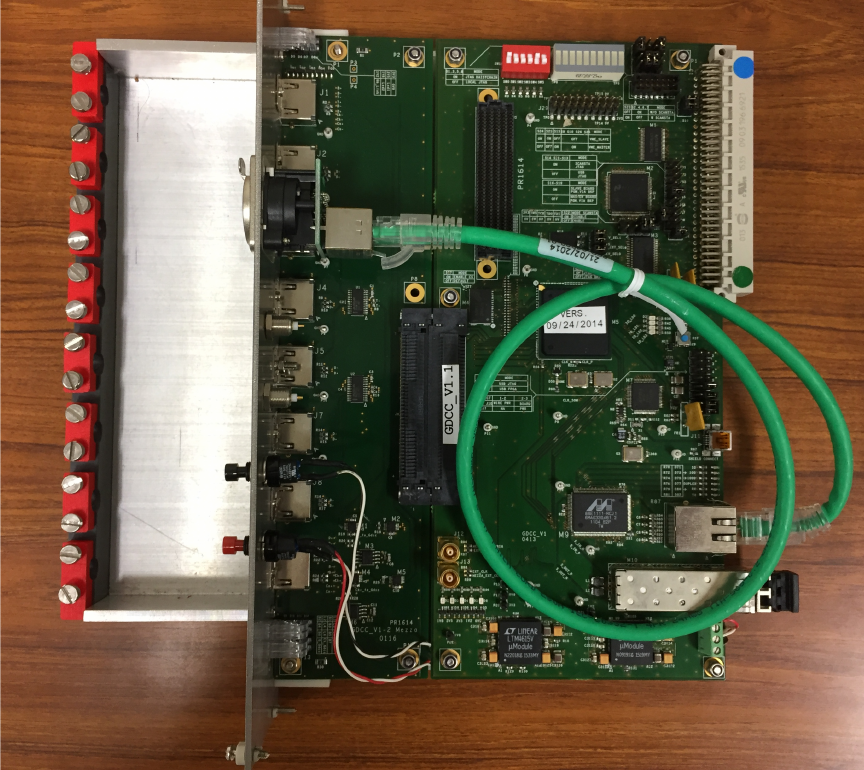
\includegraphics[width=0.7\linewidth, frame]{GDCC}
  \caption{Gigabit Data Concentrator Card (GDCC) or Clock and Control Card
    (CCC)}
\end{figure}
I have not much to add in addition to what is already in the literature quoted
in Section~\ref{sec:overview}. This is the board that I know the least about,
just because, fortunately, it just works and has never given any problem so far.

Please refer to the literature~\cite{GDCC:2012} or
Appendix~\ref{sec:gdcc-cheat-sheet} if you want/need to know more about the
GDCC.

The communication between the PC and GDCC is built on standard
Ethernet. Communication to and from it is done via RAW Ethernet packets. This is
why it doesn't need an IP address. This way communication between the DAQ PC and
the GDCC can be faster than if they traveled through the IP layer but the GDCC
must necessarily be located on the same physical LAN network as the DAQ PC.

\subsection{How to make a power supply cable}
The GDCC is build in the standard VME layout. It is meant to be plugged into a
VME crate slot for power and mechanical stability. As far as I know,
communication with the VME crate is hardware-ready but not implemented in
software yet.

In case you don't have a VME crate at hand you can easily fabricate a specific
power adapter to power up the GDCC and CCC with a standard Power Supply
Unit. The nominal voltage is DC $+5V$. The PSU must be able to supply at least
$5A$ of DC current.

For this, you need to find or buy
\begin{itemize}
\item 2 VME female connectors (96 way 2.54mm pitch). One for the GDCC and
  another for the CCC (RS reference number:
  \href{https://jp.rs-online.com/web/p/din-41612-connectors/0470443/?sra=pstk}{RS
    470-443}).
\item A breadboard to solder the connectors and the cables onto (RS reference
  number in Europe
  \href{https://uk.rs-online.com/web/p/matrix-boards/4570755/}{RS 457-0755}, RS
  reference number in Japan
  \href{https://jp.rs-online.com/web/p/matrix-boards/6647876/?sra=pstk}{RS
    664-7876}) (single side Matrix board, 2.54 pitch). You need only one boards
  that you can cut in 2 parts, one for each adapter.
\item Black and red cable unipolar cable for connections.
\item Two connectors to connect to the Power Supply (the connector type depends
  on your Power Supply and your ``taste'').
\end{itemize}

About the connection, you need to solder the pins A32,B32,C32 together and
connect these one to a red cable that you will then use for the 5V voltage.

You need to solder the pins A9, A11, A15, A17, A19, B20, B23, C9 together and
connect these one to a black cable that you will then use for the ground.

TO-DO add pictures and pinout

\section{CCC}
Clock and Control Card (CCC)

\subsection{How to convert a GDCC into a CCC}
\epigraph{Do you know how the Orcs first came into being? They were elves once,
  taken by the dark powers. Tortured and mutilated: a ruined and terrible form
  of life.}{The Lords of the Rings} All the CCC boards are produced as GDCC and
then converted in CCC by flashing a new firmware and slightly modifying the
printed board. The modification is not so complex and with a minimum effort can
be done by hand if one has the right tools.

To flash the firmware you need a Xilinx programmer like this: TO-DO

Once the firmware has been flashed it is time to modify the printed circuit. You
only need to short the R28 and R29 resistors by inserting two $0\Omega$ resistor
in the appropriate pins.
\begin{figure}[ht]
  \centering 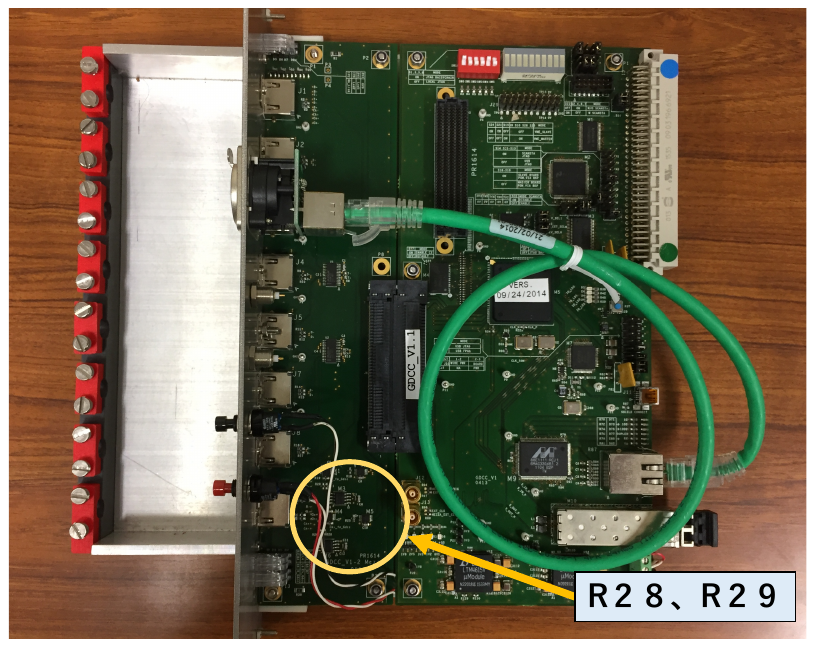
\includegraphics[width=0.5\linewidth,frame]{GDCC-CCC1}
  \caption{The position of the R28 and R29 resistors on the board.}
\end{figure}
\begin{figure}[ht]
  \centering 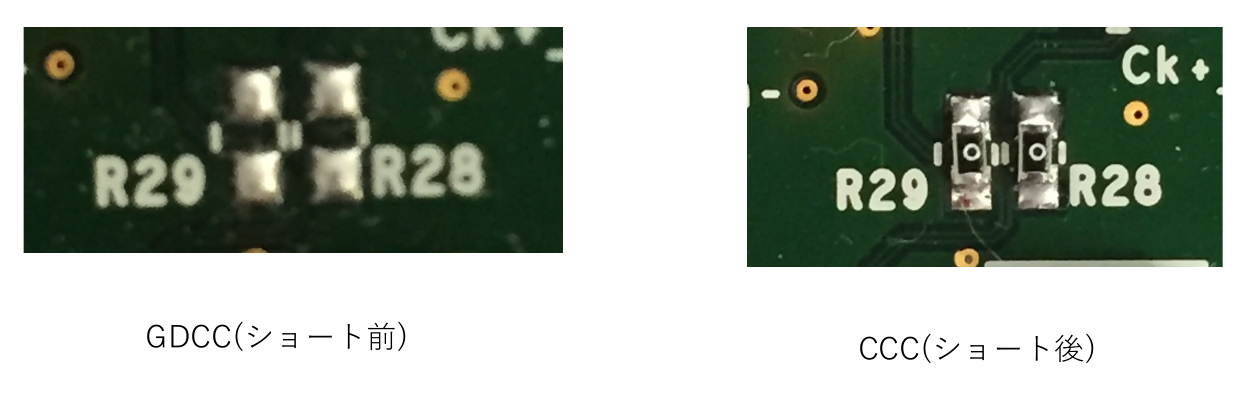
\includegraphics[width=0.8\linewidth]{GDCC-CCC2}
\end{figure}
You can solder the resistors with a traditional solder iron or with a hot air
gun. In any case you need at least two $0\Omega$ resistors of size 1608 (1.6 mm
× 0.8 mm). You can find them on the Japanese RS web-shop under the RS reference
number ``631-5667''. The full description is:
\begin{itemize}
\item \begin{CJK}{UTF8}{min}KOA 厚膜チップ抵抗器,ジャンパーチップ抵抗器, 1608サイ
    ズ, $0\Omega$, $\pm
    0$ \\
    RS品番 631-5667 メーカー型番 RK73Z1JTTD メーカー/ブランド名 KOA\end{CJK}
\item KOA thick-film resistor, jumper-chip resistor, size 1608, $0\Omega$, $\pm
  0$ \\
  RS number 631-5667 maker number RK73Z1JTTD maker/brand KOA
\end{itemize}
Anyway, the maker is not important as long as the value and size are correct.
You can solder the resistor in at least two ways. One is with a soldering
conical tip
\begin{itemize}
\item iron soldering you will also need:
  \begin{itemize}
  \item solder (remember that lead is poisonous for all life forms including
    you)
  \item tweezers
    (\href{https://www.monotaro.com/p/0840/4873/?displayId=5}{monotaro number
      TSP-26})
  \item flux (\href{https://www.monotaro.com/p/3952/8833/?displayId=5}{monotaro
      number FS20001})
  \item flux remover
    (\href{https://www.monotaro.com/p/6215/1382/?displayId=5}{monotaro number
      BS-W20B})
  \end{itemize}
\item hot air gun soldering
  (\href{https://www.monotaro.com/p/4893/0954/?displayId=5}{monotaro number
    FR810B-81}) you will also need:
  \begin{itemize}
  \item solder paste (it already contains flux)
    (\href{https://www.monotaro.com/p/1001/3097/?displayId=5}{monotaro number
      SMXB05})
  \item tweezers
  \item flux remover
  \item heat resistant tape
    (\href{https://www.monotaro.com/p/5638/8526/?displayId=5}{monotaro number
      15})
  \end{itemize}
\end{itemize}

\section{Low and High Voltage PS}
\subsection{Keithley 2400 SourceMeter}
From the Keithley 2400 SourceMeter manual:\textit{The Keithley 2400 SourceMeter
  combines a precise, low-noise, highly stable DC power supply with a low-noise,
  highly repeatable, high-impedance multimeter.}

I used this device at Yokohama National University as a High Voltage source for
my tests. This section describes how to operate this instrument from a personal
computer. Why go through the hassle of operating the Keithley from remote, if
every operation can be also performed directly from the detector front panel?
you may ask \dots The fact is that, back then, I was still in the process of
learning the Pyrame framework and I though that writing the Pyrame interface for
this instrument could be a good chance to test my comprehension of the Pyrame
code. Anyway, you may skip this section if you don't own a Keithley 2400 or you
are not interested in remotely operating it.

\subsubsection{GPIB or RS-232?}
You can connect the Keithley 2400 to a PC in two ways, each one with pros and
cons. One way is by using the GPIB port and the other is by using the RS232
port.
\begin{figure}[ht]
  \centering 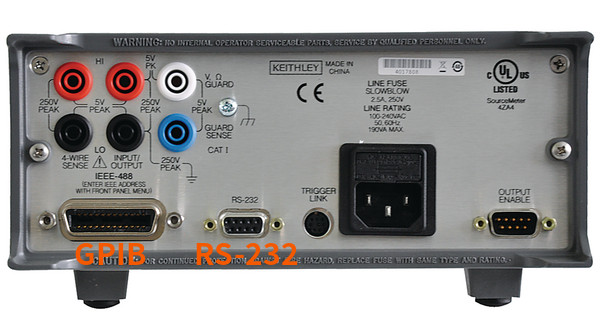
\includegraphics[width=0.7\linewidth]{keithley-2400-rear-panel}
  \caption{The Keithley 2400 SourceMeter rear panel.}\label{keithley-2400-rear-panel}
\end{figure}

The General Purpose Interface Bus (GPIB but also called IEEE-488) is a
short-range bus specification. Newer standards have largely replaced GPIB for
computer use, but it still sees some use in the test equipment field. There are
GPIB drivers for linux but they are not usually included in most distributions
repositories, so you may have to compile them yourself. Since the WAGASCI DAQ
runs on Linux I am not considering here Windows and Apple. For example, you can
find a binary package for CentOS 7 ready to install but, in the case of Ubuntu,
you have to compile it from source yourself.

To physically connect the instrument you have three options: a GPIB-to-USB
adapter, a GPIB-to-Ethernet adapter or a PCI-GPIB board. I have personally
tested only the GPIB-to-USB adapter case. The main problem with GPIB is that in
any case, it is very expensive. The average price for any of those adapters is
around 200\$ or 20000¥ on Amazon (probably much more on specialized sites).
\begin{itemize}
\item GPIB pros
  \begin{itemize}
  \item You don't need to worry about the cable pinout
  \item Adapters and cables are quite standardized so every cable and adapter
    will work just fine.
  \end{itemize}
\item GPIB cons
  \begin{itemize}
  \item You need an adapter or a PCI-GPIB card
  \item It is very expensive (both cables and adapters)
  \item It requires you to install or compile specialized drivers
  \item If you use a GPIB-to-USB adapter you are limited to 3 meters for the
    length of the USB cable
  \end{itemize}
\end{itemize}

In the case of RS-232, only a simple serial cable with DB-9 connectors is needed.
\begin{itemize}
\item RS-232 pros
  \begin{itemize}
  \item It doesn't require a specialized adapter (or a very cheap one)
    since virtually any Desktop motherboard already have a serial port (called
    sometimes COM port).
  \item Cables and adapters are quite cheap. In the case of a Desktop PC you
    can get by with very little money (20\$ or 2000¥).
  \item It doesn't required specialized drivers
  \end{itemize}
\item RS-232 cons
  \begin{itemize}
  \item Choosing the right cable and adapter is difficult because there are so
    many different types of RS-232 cables.
  \item You may need to refer to your motherboard and to the Keithley serial
    port pinout schematics to understand which is the right cable/adapter or to
    fix the adapter pinout if you bought the wrong one (like me).
  \end{itemize}
\end{itemize}
If you chose the GPIB option, you can go straight to section TO-DO to learn how
to configure and use it in the Pyrame framework.

If you chose the RS-232 option in the next subsection I will explain how to
chose the right cable and adapter and test if the pinout is correct.
\subsubsection{RS-232 connection and pinout}
The Keithley RS-232 serial port is connected to the serial port of a computer
using a straight-through RS-232 cable terminated with DB-9 connectors. Do not
use a null modem cable. The serial port uses the transmit (TXD), receive (RXD),
and signal ground (GND) lines of the RS-232
standard. Figure~\ref{RS232-pinout-instrument} shows the rear panel connector
for the RS-232 interface and the pinout for the connector.
\begin{figure}[ht]
  \centering 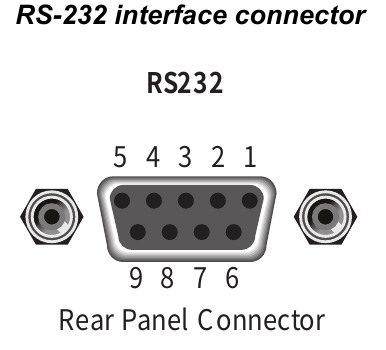
\includegraphics[width=0.4\textwidth]{RS232-pinout-connector}\hfill
  \centering 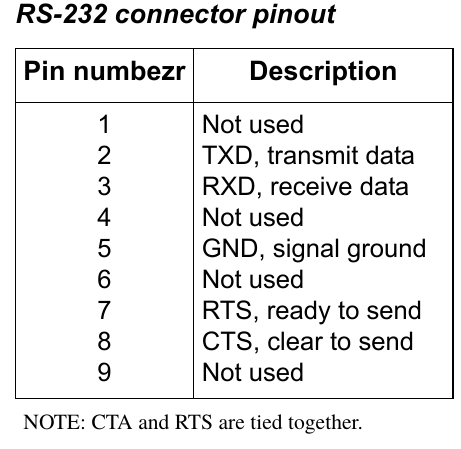
\includegraphics[width=0.4\textwidth]{RS232-pinout-instrument}
  \caption{}\label{RS232-pinout-instrument}
\end{figure}

Most desktop motherboards have a serial port (usually called COM) port like
shown in Figure~\ref{DB9-board-connection} with the relative adapter (usually to
be bought separately).
\begin{figure}[ht]
  \centering
  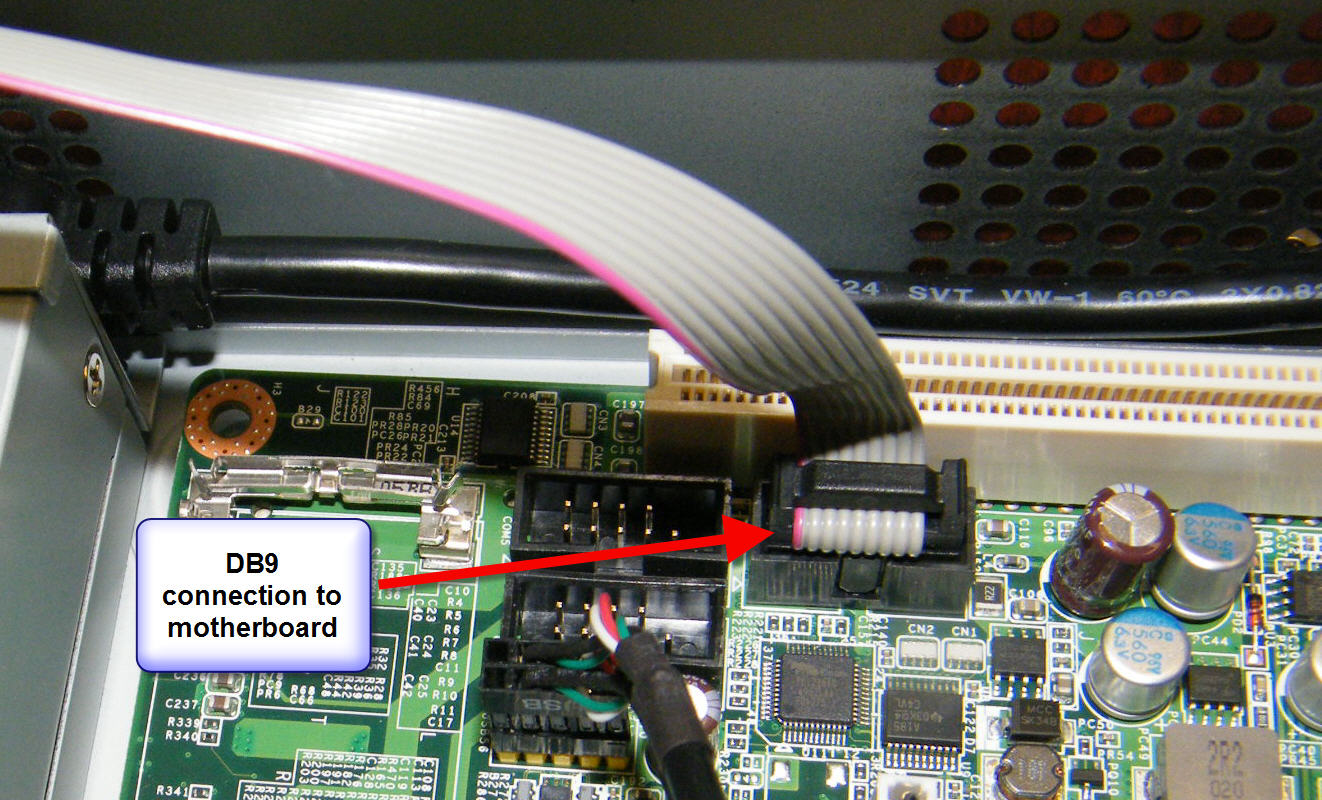
\includegraphics[width=0.55\textwidth,frame]{DB9-board-connection}\hfill
  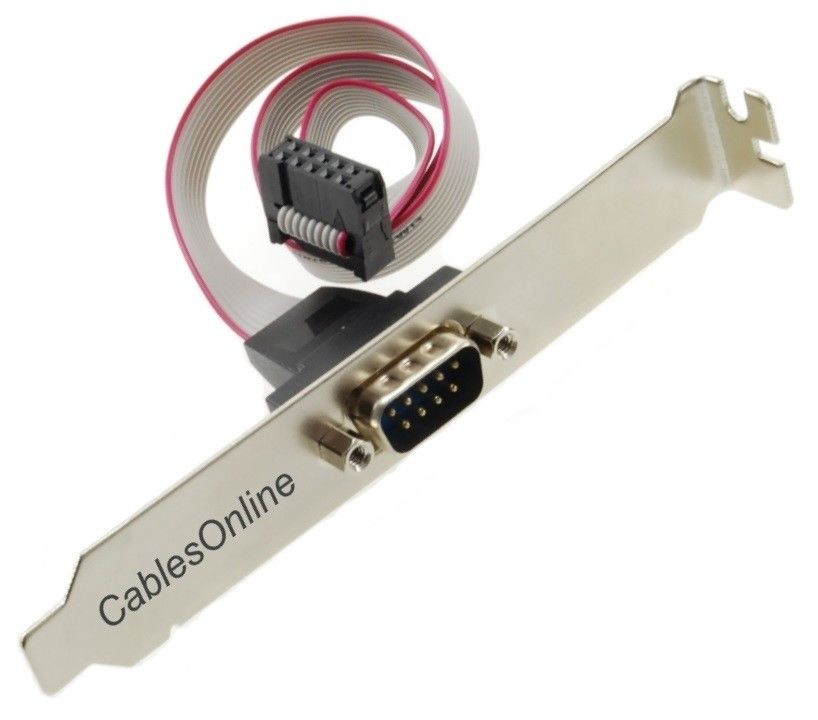
\includegraphics[width=0.4\textwidth]{RS-232-adapter}
    \caption{Serial port (COM port) on a motherboard with an adapter
    attached.}\label{DB9-board-connection}
\end{figure}

Refer to your motherboard manual for the correct pinout of the COM port. I made
the mistake of buying the wrong adapter so I had to change the wires order. For
example the motherboard that I used here is a ASUS PRIME H270 PRO and, according
to the manual, the COM port pinout is shown in Figure~\ref{RS232-pinout-PC}
\begin{figure}[H]
  \centering 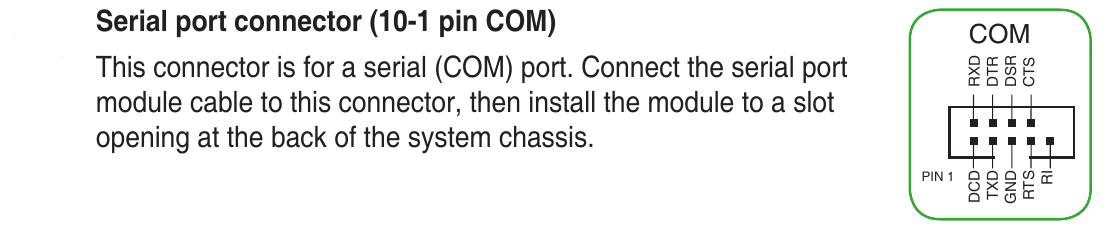
\includegraphics[width=\linewidth]{RS232-pinout-PC}
  \caption{ASUS PRIME H270 PRO motherboard COM port pinout. It may be different
    in your case!!!}\label{RS232-pinout-PC}
\end{figure}

Notice that the pin TXD (Transmit Data) on the PC side
(Figure~\ref{RS232-pinout-PC}) correspond the pin RXD (Receive Data) on the
Keithley side (Figure~\ref{RS232-pinout-instrument}) and vice versa. This is
simply because the data transmitted by the PC is received by the instrument and
vice versa. Same is for the RTS and CTS pins.
Figure~\ref{RS-232_DE-9_Connector_Pinouts} shows what is the difference between
the PC and device pinouts. Usually you only have to worry about the PC side.
\begin{figure}[ht]
  \centering 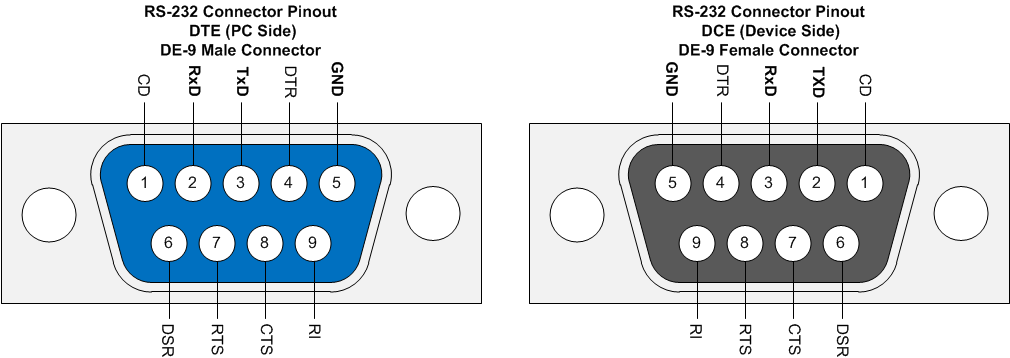
\includegraphics[width=0.9\linewidth]{RS-232_DE-9_Connector_Pinouts}
  \caption{RS-232 DE-9 Connector Pinouts}\label{RS-232_DE-9_Connector_Pinouts}
\end{figure}
I am afraid that, in any case, a certain degree of preemptive research is
unavoidable to determine which are the best cable and adapter. If you are a
WAGASCI collaborator and you are not confident in your choice, feel free to
contact me.
\subsubsection{Serial cable loopback test}
To test if the RS-232 adapter and cable are working OK, you can do a simple
loopback test. A loopback test is a simple test where you short the transmit and
receive pins of your cable or adapter (Figure~\ref{RS-232_loopback}) and try to
simultaneously send and receive some random string over the cable. Since those
pins are shorted the sent string is reflected back and received.
\begin{figure}[ht]
  \centering 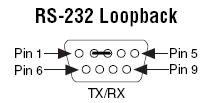
\includegraphics[width=0.4\linewidth]{RS-232_loopback}
  \caption{RS-232 loopback test: pins to short. You can use a simple
    jumper to short the pins.}\label{RS-232_loopback}
\end{figure}
Then open a two terminal on the PC and in one write:
\begin{lstlisting}
      sudo stty -F /dev/ttyS0 9600 cs8 -cstopb -parenb -echo -onlcr
      while (true) do sudo cat -A /dev/ttyS0 ; done
\end{lstlisting}
  and let it run. In the other terminal write:
\begin{lstlisting}
      echo "Hello World!" | sudo tee /dev/ttyS0
\end{lstlisting}
I have assumed that \cleanstyle{/dev/ttyS0} is the device file corresponding to
your adapter or cable. Your actual device name could be different. In case of
success you will see the same string appear in the first terminal as well.
\section{Temperature Monitors}
\section{Water Level monitor}
The USB drive must be formatted with MBR and FAT32.
\section{The WAGASCI rack}
TO-DO add picture
The WAGASCI rack is located on the south side of the WAGASCI detector as shown
in Pictures TO-DO. It is a single rack where all the acquisition electronics and
DAQ PCs are located. In this section I will explain all that there is to know
about it and how to turn it on and off. Be aware that until now the Proton
module and INGRID module data is not acquired through the WAGASCI rack but
through the INGRID one located on the SS floor.
\subsection{DAQ PC}
There are two DAQ PC in the
\subsection{ZED board}
\subsection{NIM crate}
\chapter{DAQ software}
The main software for data acquisition of the WAGASCI experiment is called Anpan
(\textbf{Acquisition Networked Program for Accelerated Neutrinos}). It is based
on the Calicoes software that was used for the Silicium Tungsten Electromagnetic
Calorimeter (SiW-ECAL) prototype of the future International Linear Collider,
developed by Frédéric Magniette and Miguel Rubio-Roy. Both Anpan and Calicoes
are based on the Pyrame framework of which they two similar implementations.

\section{Overview}
Until Summer 2018, we were using the Calicoes software without almost any
modification as the data acquisition software for the WAGASCI prototype
(i.e. Proton Module + WAGASCI water-in detector + Ingrid module).

Between the end of the WAGASCI prototype commissioning run in Summer 2018 and
the beginning of the WAGASCI Experiment Physics run in the 2019 spring, I
started my Ph.D. at YNU and I decided to further develop and improve the WAGASCI
DAQ system. So I took the decision (quite one-sidedly I have to admit) to change
the name of the acquisition software from Calicoes to Anpan (Acquisition
Networked Program for Accelerated Neutrinos), to keep these two implementations
of the Pyrame framework separated.

Since Anpan is based on Calicoes code and Calicoes is proprietary software, I am
not able to release Anpan publicly. Credit for Anpan and Calicoes goes entirely
to the original authors (Frédéric Magniette, Miguel Rubio-Roy and Thomas
Mueller). If I forgot to mention somebody please let me know.

I have chosen that name because wagashi (after which the WAGASCI experiment is
named) in Japanese means ``traditional sweets'' and anpan (a soft bun filled
with red soy beans paste) is a kind of Japanese sweet snack (even if not
strictly traditional). Anyway, I love anpan and I eat one of them almost
everyday so we can say that the development of this software was fueled mainly
by anpan. From that the name choice.

This chapter of the documentation isn't a thorough guide of all the code that
makes up anpan because much of that is already explained in the
\href{http://llr.in2p3.fr/sites/pyrame/documentation/}{Pyrame documentation
  website} and
\href{http://llr.in2p3.fr/sites/pyrame/calicoes/documentation/}{Calicoes
  documentation website}. Anyways those websites are mainly aimed at developers
who are well-versed in scientific programming and are not afraid of reading
through much of the source code. Instead, this guide is meant to be a user
manual for the physicist who just wants to use the software (and maybe only
write some simple scripts).

One must always keep in mind that most of the times scientific software is not
written by a big team of programmers with a steady job and a steady income, but
by a few researchers or worse grad students with little (or no) income
whatsoever, unsteady future prospects and a very limited budget. Because of the
lack of money and man-power, usually the first thing that get cut or reduced is
documentation (because it is not strictly necessary for the software to
run). This, as long as the original developers are also the users of the
software, has no tangible consequences. But as new physicists start to use the
software an evil-loop onsets where software is used just as-is and
works-just-because-it-works. Luckily the Calicoes and Pyrame software is
adequately documented and with this guide I would like to close the gap between
users and software even further.

\subsection{References}
There are a few published articles about the Pyrame framework. Here I am listing
all the articles that I could find. These articles are also cited throughout this
Documentation in the relevant sections.
\begin{itemize}
\item General articles about the ILC Calorimeter DAQ
  system:\cite{Gastaldi:2014vaa,Gastaldi:2014oid}
\item Articles about the Pyrame
  framework:\cite{Gastaldi:2014oid,Rubio-Roy:2015,Rubio-Roy:2017nco}
\item Websites: Pyrame~\cite{Pyrame}, Calicoes~\cite{Calicoes},
  CALICE\cite{CALICE-DAQ}
\end{itemize}

\section{Pyrame}
I won't go into detail describing the Pyrame framework since much of what I have
to say is already covered in the
\href{http://llr.in2p3.fr/sites/pyrame/documentation/}{Pyrame documentation
  website} or~\cite{Rubio-Roy:2015}. So before continuing to the following I
would suggest the reader to take a quick look there and get a rough idea of what
is happening inside of Pyrame. This section is merely intended as an appendix
and a review of the content shown there. The only real difference with the
online documentation is that, instead of trying to explain how the software
works, I will take the point of view of the user and I will only focus on how to
use Pyrame to get some work done.

First, what the user need to understand is that Pyrame is a distributed
software. This means that each part or function of Pyrame can be located on a
different machine. Each of those parts are called ``modules'' and each module
communicates with the others through the exchange of TCP/IP packets. If you
don't know what the TCP/IP protocol is you can consult the Wikipedia pages:
\href{https://en.wikipedia.org/wiki/Transmission_Control_Protocol}{TCP} and
\href{https://en.wikipedia.org/wiki/IPv4}{IP}, that should be enough.

Basically each machine able to get an IP address can open a network port through
which a certain application (or in the case of Pyrame a certain module) can
communicate and interact with the modules ``outside''. For modules residing on
the same machine the \cleanstyle{localhost=127.0.0.1} IP address must be
used. The purpose of the localhost IP address is simply to send an outgoing
packet back in. So for example if we want to reach the Configuration Module
(CMOD) that is running on the port \cleanstyle{CMOD\_PORT=9002} on the local
machine we need the only to use the couple \cleanstyle{localhost:CMOD\_PORT} or
explicitly \cleanstyle{127.0.0.1:9002}. Or if we want to communicate with the
Variables Module (VARMOD) that is running on the port
\cleanstyle{VARMOD\_PORT=9001} on another machine in the same sub-net with IP
\cleanstyle{192.168.10.100} we would address it as
\cleanstyle{192.168.10.100:9001} and so on.  The list of all the default ports
is located in \cleanstyle{/opt/pyrame/ports.txt}

There are 7 fundamental modules that must be always running during data
acquisition for Pyrame to function correctly:
\begin{itemize}
\item The Variables module: \cleanstyle{VARMOD\_PORT=9001}
\item The Configuration module: \cleanstyle{CMOD\_PORT=9002}
\item The Mount Datadir Module: \cleanstyle{MOUNTD\_PORT=9005}
\item The Acquisition-Chain Module: \cleanstyle{ACQ\_PORT=9010}
\item The Run Control Module: \cleanstyle{RC\_PORT=9014}
\item The Storage Module: \cleanstyle{STORAGE\_PORT=9020}
\end{itemize}
There may be other modules running depending on the specific configuration. The
needed modules are usually started automatically when a configuration file is
loaded so the user doesn't need to worry about that. To learn more about the
configuration file go to section TO-DO.\@

Starting from Section~\ref{sec:CMOD} I will give a short description of each of
these modules, but before that I would like to talk about the ``State Machine''.

\subsection{State Machine}
In Pyrame, the detector is always thought to be in one of four states. They are:
\begin{enumerate}
\item\label{undefined} UNDEFINED:\ The detector state has not been probed
  yet. This is the state of the detector before Pyrame has started or after it
  has ended.
\item READY:\ The detector itself is in the same UNDEFINED state as before but
  the software has been initialized and the detector configuration has been
  loaded into memory.
\item CONFIGURED or RECONFIGURED:\ The configuration has been applied to the
  detector. This means that the firmware of the various boards has been
  configured, the power supplies turned on, the voltage set up and so on. The
  detector is ready to take data.
\item\label{acquiring} ACQUIRING The detector is acquiring data.
\end{enumerate}
The principle at the base of the Pyrame workflow is that the user must go
through all the steps from~\ref{undefined} to~\ref{acquiring} in order to take
data. The software will take charge of managing all the synchronization issues.
All the transitions between machine state can be accomplished with the aid of
shell scripts called from a terminal: \cleanstyle{load\_config\_file.sh},
\cleanstyle{initialize.sh}, \cleanstyle{configure.sh}, etc\dots. It is also
possible to use the CouchDB web-GUI to manage the transitions.
\begin{figure}
  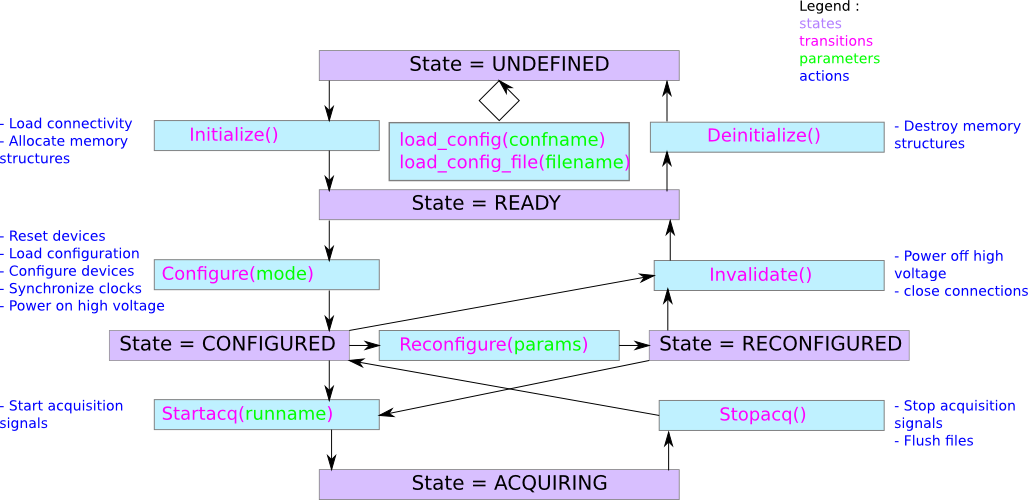
\includegraphics[frame,width=\linewidth]{state_machine.doc.png}
  \caption{Pyrame State Machine}\label{fig:state-machine}
\end{figure}

\subsection{The Configuration Module}\label{sec:CMOD}

The configuration module (called also CMOD) is in charge of many things. First,
it is dedicated to configuration storage and export.  Every Pyrame module can
register in the cmod and store its configuration parameters. The configuration
parameters and the modules themselves are organized as a tree-like structure
representing the actual structure of the detector.  TO-DO how modules can edit
the configuration?

Usually the user just load a configuration file in the cmod using the shell
script \cleanstyle{load\_config\_file.sh filename.xml}. The cmod contains at any
time a copy of the configuration of all the modules and it can generate xml
files containing all the parameters to be used with calxml.

Another role that cmod plays is to manage the transitions between different
states through the \cleanstyle{transition\_cmod} function. Again, usually this
transition is managed by shell scripts or directly by the GUI so cmod is quite
transparent to the user.

\subsection{The Variables Module}\label{sec:VARMOD}

The varmod is a centralized service that allows all the modules to share
variables for collecting statistics or sharing global information. You can store
a value associated with a name (a variable) and then get it back. You can also
make some basic operations on the variables. For more information refer to the
Pyrame documentation.

\subsection{The Acquisition-Chain Module}\label{sec:ACQ}

In my opinion, understanding completely the Pyrame Acquisition-Chain is the most
daunting task, if one really wants to know how the Pyrame software works
internally. Since I am far from an expert in that field, I will only gather here
what I have understood so far.

From the perspective of the user, reading the
\href{file:///opt/pyrame/doc/cmd_acq.html}{Pyrame documentation}, the comments
in the configuration file and the comments in the \cleanstyle{cmd\_acqpc.py}
file should be enough to get things going in almost every real-world scenario.

For the developers and more experienced users let's start by taking a look at
the graph~\ref{fig:acq-server}:
\begin{figure}[ht]
  \centering 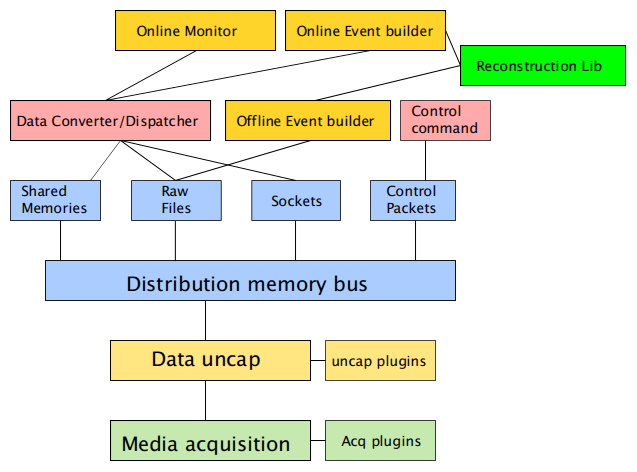
\includegraphics[frame,width=0.8\linewidth]{acq_server.doc.png}
  \caption{Pyrame State Machine}\label{fig:acq-server}
\end{figure}
I will only focus on the WAGASCI case. All the configuration regarding the
acquisition chain is done under the \cleanstyle{pcacq\_X} field in the
configuration file. If you take a pre-existing configuration file written by
myself you will find many descriptive comments in that section that hopefully
will guide you through a painless configuration.

\subsubsection{Media acquisition}
The ``media acquisition'' phase is controlled by the acquisition plugins. What
these plugins do is to ``open'' an acquisition media and get the data from
there. The acquisition media can basically be of two types: the Ethernet port
(with TCP or UDP protocols) or a raw file that was previously acquired (for
testing or debugging purposes). For a more in-depth description of every plugin
refer to \href{file:///opt/pyrame/doc/cmd_acq.html}{this page} and its
sub-pages. After the data has been acquired, it is not ready to be analyzed yet
because it contains the IP/TCP caps and it is in binary form.

You can take a look at the source code and related comments in the
\cleanstyle{anpan/cmd\_acqpc/cmd\_acqpc.py} file and in particular in the
\cleanstyle{init\_fin\_acqpc} function where every acquisition plugin is listed
and explained.

\subsubsection{Data uncap}
In this face, the acquired data is uncapped. This means that, for example in the
TCP case, the IP/TCP headers are stripped, the data integrity checked (lost or
corrupted packages) and the data content filtered (data packets or control
packets). Honestly I don't know much more than this about these plugins.

\subsubsection{Data Converter/Dispatcher}
Here the decoder library is called. For example in the case of SPIROC2D the
library path is \cleanstyle{spiroc2d\_decoder.so}. This library takes the
uncapped raw data coming from the acquisition source (for example the GDCC) and
convert it into a stream of blocks of events. These blocks are then fed to the
Online Monitor and Online Event Builder programs.  The decoder library needs to
know the channel mapping (the geometry) of the detector to associate to every
channel its position in space.

However, maybe because of some bugs or lack of time, the SPIROC2D converter for
the WAGASCI prototype commissioning run was disabled. In the
\cleanstyle{cmd\_dif.py} file the line needed to start the conversion was
commented out and function's result was always set to positive, thus completely
disabling Online Monitor capabilities of Pyrame. I am going to enable it again
and debug it (TO-DO)

Moreover, in the current Pyrame implementation only the Shared Memory and Raw
file distribution buses are implemented (check the \cleanstyle{cmd\_acq.c}
file).

\subsubsection{Online Monitor}
The WAGASCI online monitor code is contained in the
\cleanstyle{anpan/guis/om\_wagasci} folder. It is a program external to Pyrame
and WAGASCI that needs to be started by hand. It however interacts with Pyrame
under the hood. It receives the Blocks and Events created by the ``Data
Converter/Dispatcher'' face. More info about the More info can be found in
section TO-DO.\@

In Pyrame the raw data is organized in events and blocks of events. If you want
to understand in depth the WAGASCI Online Monitor it is almost mandatory that
you read this article~\cite{Rubio-Roy:2017nco}, otherwise the following
subsections won't make any sense.

\subsubsection{Events}
On a raw level, an event is just a set of hits. Each hit is roughly described by
the time, space and charge released. Other parameters may also refer to an
event. An event is described by a struct like this:
\begin{lstlisting}
      struct event {
        char **time;             // List of string containing hit times
        int time_size;           // Number of hit times
        char **space;            // List of string containing hit points
        int space_size;          // Number of hit points
        char **data;             // List of string containing various
                                 // event properties.
        int data_size;           // Number of elements in data
        char used;               // ??
        struct event *next;      // Pointer to the next event
        struct block *block;     // Pointer to the block
      };
\end{lstlisting}
Up to now the \cleanstyle{data} list contains the following elements:
\begin{itemize}
\item ``spill'': spill number.
\item ``spill\_flag'': the spill flag is set when the event happens inside of
  the beam spill time-frame. This means that the particle detected is most
  probably the result of a neutrino interaction from the neutrino beam inside or
  outside the detector.
\item ``roc'': ROC chip number.
\item ``rocchan'': ROC chip channel number.
\item ``bcid'': BCID (Bunch Crossing IDentification). Despite the misleading
  name, the BCID indicates just the number of rise time of the slow since the
  \textit{startacq} signal. More on this on TO-DO.\@
\item ``sca'': Switched Capacitor Array number.
\item ``plane'': Plane number.
\item ``channel'': Channel number.
\item ``en'': Energy (charge). This field correspond to the ADC count.
\item TDC time: ``time''
\item ``hit'': The hit flag is set if the event contains a hit. The hit may be
  due to a particle passage inside of the detector or simply by dark or electric
  noise.
\item ``gain'': The gain flag is set when we want to measure the gain. In that
  case we compare the pedestal and first hit position to calculate the gain.
\end{itemize}

\subsubsection{Blocks}
A block is a set of events bundled together according to a certain criterion
(usually the spill number or bunch number). It is described by a struct like
this:
\begin{lstlisting}
      struct block {
        int id;                  // Block identifier
        char finalized;          // ??
        int nb_events;           // Number of events in the block
        char **props;            // List of strings that can contain
                                 // various block properties as the
                                 // spill number, spill flag, etc...
        int props_size;          // Number of props strings
        char *bstr;              // ??
        struct evtstruct *es;    // This struct is used to navigate
                                 // through the various props strings
        struct event *events;    // List of events
        struct block *next;      // Pointer to the next block
      };
\end{lstlisting}
Up to now the \cleanstyle{props} list contains the following elements:
\begin{itemize}
\item spill number: ``spill''
\item spill flag: ``spill\_flag''
\end{itemize}

The ``spill\_flag'' is ``1'' during the spill time frame and ``0''
otherwise. This flag is useful to discriminate between cosmic muons and
particles coming from accelerated neutrino interactions.  For further info about
the WAGASCI spill timings refer to section TO-DO.\@

\subsection{The Run Control Module}\label{sec:RC}

TO-DO

\subsection{The Storage Module}\label{sec:STORAGE}

Storage is a Pyrame module that manages data created by other modules and its
inclusion on the RunDB.\@ For further info about the RunDB module refer to the
Pyrame documentation.

Storage allows to use a mount point and a path to transparently store data
elsewhere in the network. It also automates common tasks such as saving the
calxml configuration and a log with optional varmod variables (e.g.:\ stats) at
the same place as data files.

As far as I know there are only two kinds of storage that the Storage Module can
handle. One is the standard file on a file system and another one is a NFS share
on the network.

In the case of a standard file this is the format for the mp variable:
\begin{lstlisting}
      <param name="storage_brg_mp">file:///</param>
\end{lstlisting}
In the case of a NFS share this is the format for the mp variable:
\begin{lstlisting}
      <param name="storage_brg_mp">nfs://server/nfs</param>
\end{lstlisting}

% To autostart services (modules) when Pyrame is started edit file
% pyrame/launcher/services.txt To add default module ports edit the file
% pyrame/ports.txt

\subsection{Run and interact with Pyrame}
There are several ways to interact with Pyrame and its modules. When the
AnpanInstaller script installs Pyrame, it makes sure that Pyrame is
automatically started at every reboot. On system with
\cleanstyle{systemctl}\footnote{Both Ubuntu 18.04 and CentOS 7 use
  \cleanstyle{systemctl}} Pyrame is started as a system daemon and its execution
is controller with the \cleanstyle{systemctl} or \cleanstyle{service} shell
commands. To enable Pyrame at startup use
\begin{lstlisting}
      sudo systemctl enable pyrame
\end{lstlisting}
To disable it
\begin{lstlisting}
      sudo systemctl disable pyrame
\end{lstlisting}
To start a single time Pyrame
\begin{lstlisting}
      sudo systemctl start pyrame
\end{lstlisting}
To stop it
\begin{lstlisting}
      sudo systemctl stop pyrame
\end{lstlisting}

Moreover there are several ways to interact with Pyrame modules. If a module is
already running the simplest way to interact with it is to open a terminal and
use the command:
\begin{lstlisting}
      chkpyr2.py hostname port function parameters
\end{lstlisting}
where \cleanstyle{hostname} is the IP address of the module, for example
\cleanstyle{localhost}, \cleanstyle{port} is the port number of the module,
\cleanstyle{function} is the particular function that you want the module to
perform and \cleanstyle{parameters} are the parameters to be passed to that
function. All the public functions of the Pyrame and Anpan/Calicoes modules are
listed on the online documentations.

You can also interact with Pyrame modules from external python scripts \dots
TO-DO

\subsection{Pyrame Configuration}\label{sec:pyrame-configuration}

TO-DO


\section{Anpan}
\begin{itemize}
\item WAGASCI\_PORT=12000
\item ACQPC\_PORT=12001
\item GDCC\_PORT=12003
\item CCC\_PORT=12004
\item DIF\_PORT=12005
\item ASU\_PORT=12006
\end{itemize}

\chapter{Additional Software}
\section{ROOT 6}
ROOT is a modular scientific software framework. It provides all the
functionalities needed to deal with big data processing, statistical analysis,
visualization and storage. It is mainly written in C++ but integrated with other
languages such as Python and R\footnote{Text taken from ROOT homepage}.

This chapter is very short because much of the content that should go here is
already covered in section~\ref{root5}. The only real difference is that here we
are compiling the latest version of ROOT with the latest compilers (at the time
of writing: \today).

I am assuming here that you have never installed ROOT before. That is why we are
cloning the git repository. If you already have another installation of ROOT and
you just want to upgrade or reinstall, please make the proper modification to
these steps. I am assuming that you are capable of that.

This chapter is tailored towards Ubuntu 18.04 but it should be the same for any
other Linux distribution with some minor modifications.

\subsection{Preliminaries} First install all the packages listed in
section~\ref{packages}. Again, some of them may not be strictly needed but
cherry-picking which package is needed and which not could be very time
consuming. If you have very strict space limitations and you are somewhat forced
to install the least amount of software, I really feel sorry for you but don't
expect me to willingly help you\dots

Then make you sure you are using the last version of the compilers by issuing
\begin{lstlisting}
      gcc --version
\end{lstlisting}
The output should be
\begin{lstlisting}
      gcc (Ubuntu 7.3.0-16ubuntu3) 7.3.0
      [...]
\end{lstlisting}

\subsection{ROOT Installation}

Then follow the step~\ref{root-1} of section~\ref{root5}. Instead of
step~\ref{root-2}, type
\begin{lstlisting}
      mkdir -p $HOME/Code/ROOT/{sources,6-14-02,6-14-02-build}
      cd $HOME/Code/ROOT
\end{lstlisting}
Instead of step~\ref{root-3}, type
\begin{lstlisting}
      git clone http://github.com/root-project/root.git sources
      cd sources
      git checkout -b v6-14-02 v6-14-02
      cd ../6-14-02-build
\end{lstlisting}
Instead of step~\ref{root-4}, type
\begin{lstlisting}
      cmake -Dbuiltin_xrootd=ON
-DCMAKE_INSTALL_PREFIX=$HOME/Code/ROOT/6-14-02 ../sources
\end{lstlisting}

The following steps are the very same of section~\ref{root5} where in place of
\cleanstyle{5-34-00-patches} you just have to type \cleanstyle{6-14-02}.

\section{NEUT 5.4.0}
NEUT is a neutrino interaction simulation program library that has been
developed for the studies of the atmospheric neutrino and the accelerator
neutrinos. In this guide it is described how to compile NEUT on a Linux
machine. \textbf{NEUT 5.4.0} is the latest NEUT version at the time of writing
(\today). The author of this guide is not the NEUT author, but it is a member of
the T2K collaboration. NEUT is not an open-source software and its sources
\textbf{can be accessed only by T2K collaborators} in possession of a username
and password for the \href{https://www.t2k.org/}{T2K intranet}.

A fresh Linux installation is assumed, so, before compiling NEUT, I am showing
how to install or compile all NEUT dependencies. If you already have some of the
dependencies installed, you can safely skip the relative paragraphs. Regarding
the style of this guide, I wanted to stay on the safe side so I have explained
every step in detail. This means that the guide could appear boring and
over-repetitive to a reader well-versed in Linux software compilation and
programming and I preventively apologize for that.

\subsection{List of NEUT dependencies}\label{dep}
To compile NEUT, three main dependencies are needed:
\begin{itemize}
\item \hyperref[sec:cernlib-2005]{\textbf{CERNLIB 2005}}\\
  CERNLIB 2005 is a quite old version of \cleanstyle{cernlib}, its latest
  release being dated 2012. Unsurprisingly it is quite tricky to compile. This
  is why I have included in the present guide a complete and detailed
  walk-through to the compilation of CERNLIB 2005. There are several patches
  that need to be applied to both CERNLIB and NEUT source codes. Some of them
  were written by me, some others by Hayato-san.
\item \hyperref[root5]{\textbf{ROOT 5}}\\
  NEUT is compatible \textbf{only with ROOT 5} and not ROOT 6 yet. There are
  plans to upgrade NEUT so to make it compatible with ROOT 6, but I don't know
  if there is any progress in that direction nor if there is any ETA.\ This plan
  was announced in the last T2K meeting in May. The latest and most updated
  version of ROOT 5 is
  \href{https://github.com/root-project/root/tree/v5-34-00-patches?files=1}{ROOT
    5.34.00-patches} (it is based on ROOT 5.34.39 and the latest commit on the
  that
  \href{https://github.com/root-project/root/tree/v5-34-00-patches?files=1}{GitHub
    branch} is March 2018) and I have chosen that for my personal installation.
\item \hyperref[compiler]{\textbf{Fortran compilers}} (\cleanstyle{gfortran} and
  \cleanstyle{g77})\\
  The old fortran compiler \cleanstyle{g77} is not maintained anymore and, for
  example, it is not present in the Ubuntu repositories since the Ubuntu 8.04
  Hardy Heron (my first Ubuntu, what nostalgia). Anyway, it is still possible to
  install it in a somewhat nonstandard way as it will be shown in the following.
\end{itemize}

\subsection{NEUT compatibility}
NEUT officially supports only CentOS 7, but this doesn't mean that it cannot be
run without issues on other Linux OSes. I will introduce here 3 OSes that I have
successfully compiled NEUT onto: CentOS 7, Ubuntu 17.10 and Ubuntu 18.04. I will
show how to compile NEUT only on Ubuntu 18.04 64 bit because that is the most
delicate case and because Ubuntu 18.04 is the latest Ubuntu LST (Long Term
Support) release.
\subsubsection{CentOS 7 - TO DO}
In May 2018 Hayato Yoshinari-san, who I think is also the main developer of
\href{https://inspirehep.net/record/844435?ln=en}{NEUT}, organized a small
course about NEUT.\ Since the course was in Japanese and I am not fluent yet, I
could understand very little. Anyway, in that occasion Hayato-san provided us
with a CentOS 7 virtual machine containing all the needed dependencies to
compile and run NEUT.\ The virtual machine can be downloaded from
\href{https://tinyurl.com/y8hy9kyr}{here}. I am not sure that this link is of
public dominion, but as far as it is circulated inside the T2K collaboration
there shouldn't be any problem.  The CentOS virtual machine can be run through
Oracle \href{http://www.oracle.com/technetwork/server-storage/%
  virtualbox/downloads/index.html}{VM VirtualBox}.  The CentOS virtual machine
comes without any desktop manager. But it is possible to install it if needed (I
have installed GNOME). The user-name is \cleanstyle{neut} and the password is
\cleanstyle{neut5.4.0}. Here some relevant details about it:
\begin{center}
  \begin{tabular}{||c | c||} % chktex-file 44
    \hline % chktex-file 44
    OS & CentOS 7 \\ [0.5ex] 
    \hline\hline % chktex-file 44
    kernel & 3.10.0-693.21.1.el7.x86\_64 \\
    \hline % chktex-file 44
    gcc/g++/gfortran & 4.8.5 20150623 (Red Hat 4.8.5-16) \\ 
    \hline % chktex-file 44
    ROOT & 5.28.00h+\\
    \hline % chktex-file 44
    CERNLIB & 2005 (dated 2016/12/12) \\
    \hline % chktex-file 44
    NEUT & 5.4.0 \\ [1ex] 
    \hline
  \end{tabular}
\end{center}

\subsubsection{Ubuntu 18.04}
With the aim of writing the present guide, I wanted to test the NEUT compilation
on a fresh install. I have chosen Ubuntu 18.04 because it is the latest Ubuntu
LTS version, so in the following I will assume an Ubuntu 18.04 64 bit fresh
install.  Every other Linux distribution should be compatible after minimal
modification to some of the shell commands, particularly regarding the package
manager and the package names. Notice that I haven't used the default Ubuntu
18.04 compiler (version 7.3.0) but I have installed the old 4.8 version of
\cleanstyle{gcc}, \cleanstyle{g++} and \cleanstyle{gfortran} as shown in
subsection~\ref{compiler}.
\begin{center}
  \begin{tabular}{||c | c||} % chktex-file 44
    \hline % chktex-file 44
    OS & Ubuntu 18.04 \\ [0.5ex] 
    \hline\hline % chktex-file 44
    kernel & 4.15.0-23-generic \\ 
    \hline % chktex-file 44
    gcc/g++/gfortran & (Ubuntu 4.8.5-4ubuntu8) 4.8.5 \\
    \hline % chktex-file 44
    ROOT & 5.34.00-patches (patched version of ROOT 5.34.39) \\
    \hline % chktex-file 44
    CERNLIB & 2005 (dated 2016/12/12) \\
    \hline % chktex-file 44
    NEUT & 5.4.0 \\ [1ex] 
    \hline
  \end{tabular}
\end{center}

\subsection{Compile NEUT and its dependencies}
\subsubsection{Preliminaries}
\begin{enumerate}
\item Open a terminal or a shell. Ideally you should never close this shell from
  now until last step. If you need to close it nothing bad will happen but you
  might need to set up CERNLIB and ROOT environments again and/or come back to
  the right folder depending at which step you want to resume compilation.
\item\label{packages} First, we need to install some packages from the Ubuntu
  repositories. Some of them may be optional but I didn't have the patience to
  cherry-pick them. I have included them all just to be on the safe side. Do
  notice that it may take some time and space ($\sim$500MB).
\begin{lstlisting}
      sudo apt-get update && sudo apt-get upgrade
      sudo apt-get install build-essential git dpkg-dev cmake xutils-dev \
      g++ gcc gfortran binutils libx11-dev libxpm-dev libxft-dev libxext-dev \
      libssl-dev libpcre3-dev libglu1-mesa-dev libglew-dev \
      libmysqlclient-dev libfftw3-dev libcfitsio-dev libgraphviz-dev \
      libavahi-compat-libdnssd-dev libldap2-dev python-dev libxml2-dev \
      libkrb5-dev libgsl-dev libqt4-dev libmotif-dev libmotif-common \
      libblas-dev liblapack-dev csh tcsh gcc-4.8 g++-4.8 gfortran-4.8
\end{lstlisting}
\end{enumerate}

\subsubsection{Compilers}\label{compiler}
If you try to compile NEUT with compilers newer that 4.8, everything will still
compile fine but you will get the following error on NEUT execution time:
\begin{lstlisting}
      !!!!!!!!!!!!!!!!!!!!!!!!!!!!!!!!!!!!!!!!!!!!!!!!!!!!!!!!!!!!
      LOCB/LOCF: address 0x7f68e28cd740 exceeds the 32 bit address space
      or is not in the data segments
      This may result in program crash or incorrect results
      Therefore we will stop here
      !!!!!!!!!!!!!!!!!!!!!!!!!!!!!!!!!!!!!!!!!!!!!!!!!!!!!!!!!!!!
\end{lstlisting}
This error is ultimately connected to the \cleanstyle{FFKEY} call in
fortran. \cleanstyle{FFKEY} allows something which is read in to be an integer
or float at a later time in the run. This should not be allowed (and isn't) by
modern standards, but is still in CERNLIB and NEUT.\@

To switch between compilers, create and make executable the following shell
script
\begin{lstlisting}
      #!/bin/sh

      if [ -z "$1" ]; then
          echo "usage: $0 version" 1>&2
          exit 1
      fi

      if [ ! -f "/usr/bin/gcc-$1" ] || [ ! -f "/usr/bin/g++-$1" ] || [ ! -f "/usr/bin/gfortran-$1" ]; then
          echo "no such version gcc/g++/gfortran installed" 1>&2
          exit 1
      fi

      sudo update-alternatives --set gcc "/usr/bin/gcc-$1"
      sudo update-alternatives --set g++ "/usr/bin/g++-$1"
      sudo update-alternatives --set gfortran "/usr/bin/gfortran-$1"
\end{lstlisting}
The script accepts as the only and compulsory parameter the version of the
compiler to switch into. It is \cleanstyle{4.8} for 4.8 compilers and
\cleanstyle{7} for the 7.x compilers.

Be sure to run the script and switch to the 4.8 compiler before starting the
compilation of ROOT, CERNLIB and NEUT.\@

\subsubsection{ROOT 5}\label{root5}
As already pointed out in the introduction, at the time of writing, \textbf{NEUT
  5.4.0 is only compatible with ROOT 5}. Please refer to section~\ref{dep} for
further details about this ``issue''.  Here I will explain how to compile ROOT
5.34.00-patches starting from the source code since it is the safest way to
insure that everything is functioning correctly: if there is any incompatibility
it is usually reported at compilation time, while, if you install ROOT through
the pre-compiled binaries, any incompatibility will be uncovered only at run
time, when the errors can be more obscure and misleading to interpret.

I recommend the use of the ``three folders'' procedure to install ROOT.\ One
folder is for the source code, one for the compiling/building and one for the
final installation. The sources folder is managed entirely using git and it
contains a copy of the ROOT git repository. You can checkout the branch that you
need to compile at any time. Another folder contains the temporary building
files (such as the object files). It is effectively used only during compilation
and can be removed afterwards. It is quite heavy (about 3GB) so I usually delete
it as soon as I have installed ROOT.\@ The last folder is the installation
folder where a certain version of ROOT is installed. When running ROOT, in fact
only this folder is needed.

I am showing now how to install ROOT.\@ The following instructions are freely
taken from the following pages:
\begin{itemize}
\item \href{https://root.cern.ch/building-root}{Building root}
\item
  \href{https://d35c7d8c.web.cern.ch/root-version-v5-34-00-patch-release-notes}%
  {ROOT v5-34-00-patch release-notes}
\item \href{https://root.cern.ch/build-prerequisites}{Build prerequisites}
\end{itemize}

\begin{enumerate}[resume]
\item Open a terminal if not already opened.
\item\label{root-1} Then install some fonts required by ROOT%
\begin{lstlisting}
      sudo apt install xfstt xfsprogs t1-xfree86-nonfree ttf-xfree86-nonfree \
      ttf-xfree86-nonfree-syriac xfonts-75dpi xfonts-100dpi
\end{lstlisting}
  You can optionally install the following packets to have a more thorough ROOT
  installation. They are by no means mandatory. I honestly have no idea what
  many of these packages do. I just hate dealing with missing dependencies when
  I run software.
\begin{lstlisting}
      sudo apt install libgif-dev libtiff-dev libjpeg-dev liblz4-dev \
      liblzma-dev libgl2ps-dev libpostgresql-ocaml-dev libsqlite3-dev \
      libpythia8-dev davix-dev srm-ifce-dev libtbb-dev python-numpy
\end{lstlisting}
  
\item\label{root-2} Create two directories that will contain the ROOT source
  code and the compiled code. You can change the paths as you wish, but then you
  have to remember to change all the references and links in the following
  accordingly. You may also need to modify the patches since they include these
  paths.
\begin{lstlisting}
      mkdir -p $HOME/Code/ROOT/{sources,5-34-00-patches,5-34-00-patches-build}
      cd $HOME/Code/ROOT
\end{lstlisting}
\item\label{root-3} Clone the ROOT source code into the sources directory using
  git and then:
\begin{lstlisting}
      git clone http://github.com/root-project/root.git sources
      cd sources
      git checkout -b v5-34-00-patches origin/v5-34-00-patches
      cd ../5-34-00-patches-build
\end{lstlisting}
\item\label{root-4} Execute the cmake command on the shell.
\begin{lstlisting}
      cmake -Dbuiltin_xrootd=ON -DCMAKE_INSTALL_PREFIX=$HOME/Code/ROOT/5-34-00-patches ../sources
\end{lstlisting}
  CMake will detect your development environment, perform a series of test and
  generate the files required for building ROOT.\@
\item After CMake has finished running, start the build from the build
  directory:
\begin{lstlisting}
      cmake --build . --target install
\end{lstlisting}
  On UNIX systems (with make or ninja) you can speedup the build with%
\begin{lstlisting}
      cmake --build . --target install -- -jN
\end{lstlisting}
  where N is the number of available cores.
\item Now you can safely remove the build directory if you need that space.
\begin{lstlisting}
      cd
      rm -Rf $HOME/Code/ROOT/5-34-00-patches-build
\end{lstlisting}

\item Every time that you run ROOT, you need to setup the environment. There are
  at least three ways to do that, more ore less automated.
  \begin{itemize}
  \item One is to run the command%
\begin{lstlisting}
      source $HOME/Code/ROOT/5-34-00-patches/bin/thisroot.sh
\end{lstlisting}
    Every time it is needed.
  \item Another way is to define an alias in the \cleanstyle{.bash\_aliases}
    file or in the \cleanstyle{.bashrc} file. For instance I have set
\begin{lstlisting}
      alias root5='source $HOME/Code/ROOT/5-34-00-patches/bin/thisroot.sh'
      alias root6='source $HOME/Code/ROOT/6-12-06/bin/thisroot.sh'
\end{lstlisting}
    To quickly switch between different ROOT versions.
  \item Alternatively one can set up the correct root environment at boot by
    inserting the following lines in the \cleanstyle{.profile} file
\begin{lstlisting}
      # set the needed environment variables, PATH and LD_LIBRARY_PATH for root
      if [ -f "${HOME}/Code/ROOT/5-34-00-patches/bin/thisroot.sh" ] ; then
      source ${HOME}/Code/ROOT/5-34-00-patches/bin/thisroot.sh
      fi
\end{lstlisting}
    Then every shell will have that version of root as default.
  \end{itemize}
\item Before using root, remember to reboot (to reload the fonts). Then you can
  ROOT with the command \cleanstyle{root}.
\end{enumerate}

\subsubsection{CERNLIB 2005}\label{sec:cernlib-2005}
The following procedure was freely taken from the three reference web pages:
\begin{itemize}
\item \href{https://www.t2k.org/asg/xsec/niwgdocs/neut/install_neut}{NEUT
    installation}
\item
  \href{https://www-zeuthen.desy.de/linear_collider/cernlib/new/cernlib_2005.html}%
  {CERNLIB installation }
\item \href{http://seanelvidge.com/2017/01/install-g77-on-ubuntu-14-04/}{g77
    installation}
\end{itemize}
\begin{enumerate}[resume]
\item Create a new folder for CERNLIB and move to it. In the following I am
  assuming that you won't leave that folder until the CERNLIB compilation is
  complete.
\begin{lstlisting}
      mkdir $HOME/Code/CERNLIB
      cd $HOME/Code/CERNLIB
\end{lstlisting}
\item CERNLIB uses a different naming for make. I suppose this is due to small
  differences in naming conventions between UNIX and Linux (g-nu).%
\begin{lstlisting}
      sudo ln -s /usr/bin/make /usr/bin/gmake
\end{lstlisting}
\item The following commands add the hardy repositories to the
  \cleanstyle{sources.list} file and install \cleanstyle{g77}. This step is
  needed to download and install the fortran \cleanstyle{g77} compiler. It is
  advisable to comment or remove these lines after the \cleanstyle{g77}
  installation.%
\begin{lstlisting}
      sudo tee -a /etc/apt/sources.list << END

      # Old hardy repository needed to install g77
      # It is recommended to comment or remove following lines after g77 installation
      
      deb [trusted=yes] http://old-releases.ubuntu.com/ubuntu/ hardy universe
      deb-src [trusted=yes] http://old-releases.ubuntu.com/ubuntu/ hardy universe
      deb [trusted=yes] http://old-releases.ubuntu.com/ubuntu/ hardy-updates universe
      deb-src [trusted=yes] http://old-releases.ubuntu.com/ubuntu/ hardy-updates universe
      END
      sudo apt-get update && sudo apt-get install g77
\end{lstlisting}
\item Now it is time to solve a couple of bugs of the \cleanstyle{g77}
  compiler. This is quite an old and now largely obsolete compiler. For this
  reason many adjustments are needed to get it working. You may need to modify
  the code below if your system libraries path or your gcc compiler version are
  different. For more information and troubleshooting please consider visiting
  \href{http://seanelvidge.com/2017/01/install-g77-on-ubuntu-14-04/}{this page}.

  The following command will create a symbolic link of a library that
  \cleanstyle{g77} would not able to find otherwise.
\begin{lstlisting}
      sudo ln -s /usr/lib/gcc/x86_64-linux-gnu/7/libgcc_s.so /usr/lib/x86_64-linux-gnu/
\end{lstlisting}
\item Then let us set up the \cleanstyle{LIBRARY\_PATH} environment
  variable. This must be done every time you want to use the \cleanstyle{g77}
  compiler.
\begin{lstlisting}
      export LIBRARY_PATH="/usr/lib/x86_64-linux-gnu:\$LIBRARY_PATH"
\end{lstlisting}
  If you want to avoid issuing the previous command every time, you can do the
  following:
\begin{lstlisting}
      tee -a $HOME/.profile << END

      # set LIBRARY_PATH so it includes x86_64-linux-gnu if it exists
      if [ -d "/usr/lib/x86_64-linux-gnu" ] ; then
      LIBRARY_PATH="/usr/lib/x86_64-linux-gnu:\$LIBRARY_PATH"
      export LIBRARY_PATH
      fi
      END
\end{lstlisting}
  
\item Download all the CERNLIB 2005 source code archives:%
\begin{lstlisting}
wget http://www-zeuthen.desy.de/linear_collider/cernlib/new/cernlib-2005-all-new.tgz
\end{lstlisting}
\begin{lstlisting}
wget http://www-zeuthen.desy.de/linear_collider/cernlib/new/cernlib.2005.corr.2014.04.17.tgz
\end{lstlisting}
\begin{lstlisting}
wget http://www-zeuthen.desy.de/linear_collider/cernlib/new/cernlib.2005.install.2014.04.17.tgz
\end{lstlisting}
\item Extract the downloaded files:
\begin{lstlisting}
      tar -zxvf cernlib-2005-all-new.tgz
      cp cernlib.2005.corr.2014.04.17.tgz cernlib.2005.corr.tgz
      tar -zxvf cernlib.2005.install.2014.04.17.tgz
\end{lstlisting}

\item Download my patched version of the old \cleanstyle{patchy 4} source code
  and substitute it with the non patched one. I am not sure if the
  \cleanstyle{patchy} suite is really necessary for NEUT but it is better to
  have and not need it than need it and not have.
\begin{lstlisting}
rm patchy4.tar.gz
wget https://www.dropbox.com/s/n7n1wiivn1noets/patchy4.tar.gz
\end{lstlisting}

  
\item Download and check the patch:
\begin{lstlisting}
      wget https://www.dropbox.com/s/loa53mklvotzsvj/jojo-CERNLIB.patch
      cp Install_cernlib Install_cernlib.backup
      patch -p0 --dry-run < jojo-CERNLIB.patch
\end{lstlisting}
\item If there isn’t any error, patch the installation script
\begin{lstlisting}
      patch -p0 < jojo-CERNLIB.patch
\end{lstlisting}
\item Now you can compile CERNLIB.\@
\begin{lstlisting}
      ./Install_cernlib
\end{lstlisting}
\item Check that the compilation process went well by looking for errors in the
  log files in \cleanstyle{2005/build/log}
\begin{lstlisting}
      grep ./2005/build/log -R -i -e "error [0-9]" | grep -v ZDROP | grep -v ZBOOKN
\end{lstlisting}
\item Finally set up the CERNLIB environment for the next section.
\begin{lstlisting}
      source cernlib_env
\end{lstlisting}
\end{enumerate}

\subsection{NEUT 5.4.0}
\begin{enumerate}[resume]
\item If you are continuing from the same terminal as the previous section, you
  don't need this step. Otherwise open the terminal and issue the following
  commands to setup the NEUT compilation environment:
\begin{lstlisting}
      source $HOME/Code/ROOT/5-34-00-patches/bin/thisroot.sh
      source $HOME/Code/CERNLIB/cernlib_env
\end{lstlisting}
\item Create the NEUT folder and move to it.
\begin{lstlisting}
      mkdir $HOME/Code/NEUT
      cd $HOME/Code/NEUT
      export NEUT_ROOT=$HOME/Code/NEUT
\end{lstlisting}
\item Download the NEUT source code from
  \href{https://www.t2k.org/asg/xsec/niwgdocs/neut/NEUT5.4.0}{this link}. To
  download the file it is necessary to insert one's own T2K credentials. Then
  move the downloaded archive in the NEUT folder. During the download don't
  close the terminal. Go back to the terminal and issue:
\begin{lstlisting}
      cd $HOME/Code/NEUT
      mv neut_5.4.0_20180120.tar.gz neut_5.4.0_20180120.tar
      tar -xvf neut_5.4.0_20180120.tar
      mv neut_5.4.0/src ./src
      rmdir neut_5.4.0
\end{lstlisting}
\item Download and check the patches
\begin{lstlisting}
      cd src/neutsmpl
      wget https://www.dropbox.com/s/dxyjk5fzw0vuv85/jojo-NEUT-1.patch
      wget https://www.dropbox.com/s/ew07kn9duzvhqtt/jojo-NEUT-2.patch
      patch -p0 --dry-run < jojo-NEUT-1.patch
      patch -p0 --dry-run < jojo-NEUT-2.patch
\end{lstlisting}
\item If there aren't errors, apply the patches:
\begin{lstlisting}
      patch -p0 < jojo-NEUT-1.patch
      patch -p0 < jojo-NEUT-2.patch
\end{lstlisting}
\item Finally compile NEUT.\@ All should be fine now.
\begin{lstlisting}
      ./Makeneutsmpl.csh
\end{lstlisting}
\end{enumerate}

\chapter{Appendix}
\section{GDCC cheat-sheet}\label{sec:gdcc-cheat-sheet}
This cheat-sheet is intended for debug only. Normal users (myself included)
should not need to care about this. I have included it in the appendix just in
case I would need it in future (but I really hope not). The GDCC is built on
standard Ethernet. Communication to and from it is done via RAW Ethernet
packets:
\subsection{Fast command packet format}
Fast commands are generated via two mechanisms. The first is in direct response
to various hardware inputs from the CCC into the GDCC and the second is manually
via the GDCC \textrightarrow COMPUTER link.

When done via this method the packet used is smaller than the normal GDCC packet
format, and is processed separately.
\begin{table}[ht]
  \centering \resizebox{\textwidth}{!}{ \bgroup
    \def\arraystretch{1.5}% 1 is the default, change whatever you need
    \begin{tabular}{|c|c|c|c|c|c|c|c|c|c|}
      \hline
      Dst MAC & Src MAC & Ethernet Type & Command\_Word & DIF Link & %
                                                                     Comma &  Data & parity & PAD & CRC32 \\ %
      \hline
      6 Bytes & 6 Bytes & 2 bytes & 2 Bytes & 2 Bytes & 1 Byte & %
                                                                 1 Byte & 2 Bytes & Pad to min Ethernet size & 4 bytes \\
      \hline
    \end{tabular}
    \egroup }
  \caption{Fast command packet format}
\end{table}

\begin{itemize}
\item Ethernet type: set to \texttt{0x0809} for Fast Command. These are
  generally not used in the real world, so we chose them at random. Packets with
  a different Ethernet Type will be ignored.
\item Command word: set to a constant \texttt{0xFA57}. Future operations may use
  a different Command\_Word for other usage cases.
\item DIF Link: A mask which defines which port the command is for. A value of
  \texttt{0xFFFF} would be used as a broadcast to all currently active DIF
  links.
\item Comma: comma character to use
\item Data: defines which byte to send as the data byte.
\item Parity: is a simple check, the bits of this are defined as follows
  \begin{table}[H]
    \centering \bgroup
    \def\arraystretch{1.3}% 1 is the default, change whatever you need
    \begin{tabular}{|c|c|}
      \hline
      \textbf{Bit} & \textbf{Data Used} \\
      \hline
      0 & Lower 8 bits of Command\_Word \\
      \hline
      1 & Upper 8 bits of Command\_Word \\
      \hline
      2 & Lower 8 bits of DIF\_Link \\
      \hline
      3 & Upper 8 bits of DIF\_Link \\
      \hline
      4 & Comma \\
      \hline
      5 & Data \\
      \hline
    \end{tabular}
    \egroup
  \end{table}
  We use an Even Parity scheme, and the reason for using this is that the
  command is recognised almost as soon as the parity is validated, rather than
  waiting for the full CRC32 to be verified.
\end{itemize}


\subsection{GDCC packet format}
\begin{table}[ht]
  \centering \resizebox{\textwidth}{!}{ \bgroup
    \def\arraystretch{1.5}% 1 is the default, change whatever you need
    \begin{tabular}{|c|c|c|c|c|c|c|c|c|c|}
      \hline
      Dst MAC & Src MAC & Ethernet Type & GDCC\_type & GDCC\_modifier %
      & GDCC\_pktID  & GDCC\_dataLength & GDCC\_Data & PAD CRC32 \\
      \hline
      6 Bytes & 6 Bytes & 2 bytes & 2 Bytes & 2 Bytes & 2 Byte & %
                                                                 2 Byte  & Variable Pad to min Ethernet size & 4 bytes \\
      \hline
    \end{tabular}
    \egroup }
  \caption{GDCC packet format}
\end{table}

\begin{itemize}
\item Ethernet type:
  \begin{itemize}
  \item \texttt{0x0810}: GDCC data pkt
  \item \texttt{0x0811}: DIF data pkt
  \end{itemize}
\item GDCC type: split in 2 bytes (not all are defined)
  \begin{itemize}
  \item Upper (Sub System Encoding):
    \begin{itemize}
    \item \texttt{0x00}: GDCC registers (Both directions)
    \item \texttt{0x01}: DIF transport (Both directions)
    \item \texttt{0x02}: Diagnose memory (Both directions)
    \item \texttt{0xFF}: GDCC pkt generator (GDCC \textrightarrow PC)
    \end{itemize}
  \item Lower (Operation Encoding):
    \begin{itemize}
    \item \texttt{0x00}: GDCC PktGenData (GDCC \textrightarrow PC)
    \item \texttt{0x01}: Write from PC to GDCC (PC \textrightarrow GDCC)
    \item \texttt{0x02}: Read from PC to GDCC (PC \textrightarrow GDCC)
    \item \texttt{0x03}: Write ACK (GDCC \textrightarrow PC)
    \item \texttt{0x04}: Read reply from GDCC to PC (GDCC \textrightarrow PC)
    \item \texttt{0x05}: Read NACK (GDCC \textrightarrow PC)
    \item \texttt{0x08}: pkt\_DIF from PC to DIF (PC \textrightarrow DIF)
    \item \texttt{0x09}: pkt\_DIF from DIF to PC (DIF \textrightarrow PC)
    \item \texttt{0xFF}: GDCC Saw Bad Packet (GDCC \textrightarrow PC)
    \end{itemize}
  \end{itemize}
\item GDCC modifier: is used to indicate things such as which DIF link a DIF
  packet should be sent down, that is currently the only use of
  it. \texttt{0xFFFF} indicates a broadcast down all DIF links that are
  currently operational.
\item GDCC pktID : This is used to track Replies to things. For example a any
  GDCC register operations will result in a reply, these replies will have the
  same PktID in them.
\item GDCC data length: is a measure of how many objects there will be in the
  GDCC Data array. For Register operations on the GDCC it is the total number of
  GDCC Register Packets that follow. For DIF operations it is the Number of DIF
  Packets that follow. For DIF Event data it is the Number of Event Packets that
  follow.
\item CRC32: This is not really a user accessible data field. Normally the MAC
  layer on the Ethernet card will add this, and will strip it on received
  packets. However, depending on the operation it may or may not be visible and
  so is included in this definition for completeness. Any packets the fail the
  CRC32 check on RX at the GDCC will be silently dropped.
\end{itemize}

\subsection{GDCC Register Packet Format }
Access to GDCC registers is done via the following sub packet type.
\begin{table}[ht]
  \centering \bgroup
  \def\arraystretch{1.5}% 1 is the default, change whatever you need
  \begin{tabular}{|c|c|}
    \hline
    Address & Data \\
    \hline
    2 Bytes & 4 Bytes \\
    \hline
  \end{tabular}
  \egroup
\end{table}
Address is 16 bits, and in general fill all unused data with 0x0 Data is 32
bits, even though most registers are 16. This is to allow future expansion.

Lower bits of data are used first, so a register that returns < 32 bits will
return it in the lower bits of the data space, the same for writes.

When performing a Read the packet must still include the space for the data,
even though it will be over written by the GDCC internal processing. This just
makes things more symmetric for both reads and writes.

You can pack as many register sub packets as you want into an
GDCC\_packet. However, they will all be of the same type, eg, all READ or all
WRITE, you cannot currently mix them.

\subsection{GDCC DIF Event Packet Format}

When Events come into the GDCC from the DIF they are wrapped in an GDCC packet
before being sent onward to the COMPUTER. They are dropped verbatim into the
GDCC\_Data block of the packet. The GDCC-DIF Link CRC is retained, so that
software can check it if needed.

\begin{itemize}
\item GDCC\_Type: Will have the upper portion set to DIF Transport and the lower
  8 bits set to show which DIF Link it came from.
\item GDCC\_PktID: Will be the serial number of the packet, which will increase
  each time, allowing some way to see if there are missing ones.
\item GDCC\_DataLength: Will show the number of encapsulated DIF Packets
\end{itemize} Future enhancement might be the addition of a flag to say if the
packet from the DIF passed the CRC or not.

\subsection{GDCC Memory Map}
Memory access's to registers inside the GDCC are done using a 16bit
address. This address is then subdivided into a Block and Register range The
upper 4 bits define the Block. The lower 12 define the Register.

\begin{table}[H]
  \centering \bgroup
  \def\arraystretch{1.3}% 1 is the default, change whatever you need
  \begin{tabular}{|c|c|c|}
    \hline
    \textbf{Block} & \textbf{Address} & \textbf{Register} \\
    \hline
    \texttt{0x1} & \texttt{0x000} & DIF\_LINK\_TX\_EN \\
                   & \texttt{0x002} & DIF\_LINK\_RX\_EN \\
                   & \texttt{0x004} & DIF\_LINK\_RTT \\
                   & \texttt{0x006} & DIF\_LINK\_AUTONEG\_PAUSE \\
                   & \texttt{0x008} & DIF\_LINK\_RESTART \\
                   & \texttt{0x00A} & DIF\_LINK\_STATUS1 \\
                   & \texttt{0x00B} & DIF\_LINK\_STATUS2 \\
                   & \texttt{0x00E} & DIF\_LINK\_NO\_SIGNAL \\
                   & \texttt{0x010} & DIF\_LINK\_DELAY1 \\
                   & \texttt{0x011} & DIF\_LINK\_DELAY2 \\
                   & \texttt{0x012} & DIF\_LINK\_DELAY3 \\
                   & \texttt{0x013} & DIF\_LINK\_DELAY4 \\
                   & \texttt{0x018} & DIF\_LINK\_RTT1 \\
                   & \texttt{0x019} & DIF\_LINK\_RTT2 \\
                   & \texttt{0x01A} & DIF\_LINK\_RTT3 \\
                   & \texttt{0x01B} & DIF\_LINK\_RTT4 \\
                   & \texttt{0x020} & DIF\_LINK\_RTT\_DONE \\
                   & \texttt{0x022} & DIF\_LINK\_LOCKED \\
                   & \texttt{0x024} & DIF\_LINK\_DCM \\
    \hline
    \texttt{0x2} & & \\
    \hline
    \texttt{0x3} & & \\
    \hline
    \texttt{0x4} & \texttt{0x000} & GDCC\_ENABLES \\
                   & \texttt{0x001} & GDCC\_TX\_MUX\_COUNT \\
                   & \texttt{0x006} & GDCC\_DIF\_DATA\_MAC\_L \\
                   & \texttt{0x007} g& GDCC\_DIF\_DATA\_MAC\_M \\
                   & \texttt{0x008} & GDCC\_DIF\_DATA\_MAC\_H \\
                   & \texttt{0x00E} & GDCC\_REVISION \\
                   & \texttt{0x00F} & GDCC\_VERSION \\
                   & \texttt{0x010} & GDCC\_PKTGEN\_CONTROL \\
                   & \texttt{0x011} & GDCC\_PKTGEN\_SIZE \\
                   & \texttt{0x012} & GDCC\_PKTGEN\_COUNT \\
                   & \texttt{0x013} & GDCC\_PKTGEN\_DELAY \\
                   & \texttt{0x014} & GDCC\_PKTGEN\_SEED \\
                   & \texttt{0x015} & GDCC\_PKTGEN\_TXCOUNT \\
                   & \texttt{0x016} & GDCC\_PKTGEN\_MAC\_L \\
                   & \texttt{0x017} &  GDCC\_PKTGEN\_MAC\_M \\
                   & \texttt{0x018} & GDCC\_PKTGEN\_MAC\_H \\
    \hline
  \end{tabular}
  \egroup
\end{table}
\printbibliography
\end{document}

%%% Local Variables:
%%% TeX-master: t
%%% End:
